\documentclass[a4paper,twoside]{article}
\usepackage[T1]{fontenc}
\usepackage[bahasa]{babel}
\usepackage{graphicx}
\usepackage{graphics}
\usepackage{float}
\usepackage[cm]{fullpage}
\pagestyle{myheadings}
\usepackage{etoolbox}
\usepackage{setspace} 
\usepackage{lipsum} 
\usepackage{url}
\setlength{\headsep}{30pt}
\usepackage[inner=2cm,outer=2.5cm,top=2.5cm,bottom=2cm]{geometry} %margin
% \pagestyle{empty}


\makeatletter
\renewcommand{\@maketitle} {\begin{center} {\LARGE \textbf{ \textsc{\@title}} \par} \bigskip {\large \textbf{\textsc{\@author}} }\end{center} }
\renewcommand{\thispagestyle}[1]{}
\markright{\textbf{\textsc{Laporan Perkembangan Pengerjaan Skripsi\textemdash Sem. Ganjil 2015/2016}}}

\onehalfspacing
 
\begin{document}
\def\bibname{Daftar Referensi}
\title{\@judultopik}
\author{\nama \textendash \@npm} 

%ISILAH DATA DATA BERIKUT INI:
\newcommand{\nama}{Herfan Heryandi}
\newcommand{\@npm}{2012730012}
\newcommand{\tanggal}{06/10/2015} %Tanggal pembuatan dokumen
\newcommand{\@judultopik}{IT STUDENT PORTAL: PEMANFAATAN \textit{WEB SCRAPING} UNTUK KUSTOMISASI PORTAL AKADEMIK MAHASISWA} % Judul/topik anda
\newcommand{\kodetopik}{PAS3904}
\newcommand{\jumpemb}{1} % Jumlah pembimbing, 1 atau 2
\newcommand{\pembA}{Pascal Alfadian}
\newcommand{\pembB}{-}
\newcommand{\semesterPertama}{39 - Ganjil 15/16} % semester pertama kali topik diambil, angka 1 dimulai dari sem Ganjil 96/97
\newcommand{\lamaSkripsi}{1} % Jumlah semester untuk mengerjakan skripsi s.d. dokumen ini dibuat
\newcommand{\kulPertama}{Skripsi 1} % Kuliah dimana topik ini diambil pertama kali
\newcommand{\tipePR}{B} % tipe progress report :
% A : dokumen pendukung untuk pengambilan ke-2 di Skripsi 1
% B : dokumen untuk reviewer pada presentasi dan review Skripsi 1
% C : dokumen pendukung untuk pengambilan ke-2 di Skripsi 2

% Dokumen hasil template ini harus dicetak bolak-balik !!!!

\maketitle

\pagenumbering{arabic}

\section{Data Skripsi} %TIDAK PERLU MENGUBAH BAGIAN INI !!!
Pembimbing utama/tunggal: {\bf \pembA}\\
Pembimbing pendamping: {\bf \pembB}\\
Kode Topik : {\bf \kodetopik}\\
Topik ini sudah dikerjakan selama : {\bf \lamaSkripsi} semester\\
Pengambilan pertama kali topik ini pada : Semester {\bf \semesterPertama} \\
Pengambilan pertama kali topik ini di kuliah : {\bf \kulPertama} \\
Tipe Laporan : {\bf \tipePR} -
\ifdefstring{\tipePR}{A}{
			Dokumen pendukung untuk {\BF pengambilan ke-2 di Skripsi 1} }
		{
		\ifdefstring{\tipePR}{B} {
				Dokumen untuk reviewer pada presentasi dan {\bf review Skripsi 1}}
			{	Dokumen pendukung untuk {\bf pengambilan ke-2 di Skripsi 2}}
		}

\section{Detail Perkembangan Pengerjaan Skripsi}
Detail bagian pekerjaan skripsi sesuai dengan rencana kerja/laporan perkembangan terakhir :
	\begin{enumerate}
		%NOMOR 1%
		\item Melakukan studi mengenai \textit{library} jsoup, Chrome DevTools, Play Framework, SIA Models, dan CSS \textit{Selector}.\\
		{\bf status :} Ada sejak rencana kerja skripsi kecuali SIA Models dan CSS \textit{Selector}.\\
		{\bf hasil :} \\
		\begin{enumerate}
			
		
\item \textbf{jsoup}

\textit{Web scraping} adalah teknik mendapatkan informasi dari sebuah situs web secara otomatis\cite{Vargiu:2013}. Dalam bahasa Java, \textit{web scraping} dapat diimplementasikan menggunakan \textit{library} jsoup\cite{jsoup}. API yang disediakan oleh jsoup dapat digunakan untuk mengekstrak dan memanipulasi data HTML. 

Bagian berikut menjelaskan beberapa kelas dari jsoup.

\textbf{Jsoup}

Kelas ini merupakan inti untuk mengakses fungsi jsoup. Seluruh \textit{method} dalam kelas ini merupakan \texttt{static} \textit{method} sehingga kelas ini tidak perlu dikonstruksi. Salah satu \textit{method} yang dimiliki kelas ini adalah sebagai berikut:
\begin{itemize}
	\item \textbf{public static Connection connect(String url)} \\
		Berfungsi untuk membuat koneksi baru dengan suatu situs web. \\
		\textbf{Parameter:}
		\begin{itemize}
			\item \textbf{url} URL situs web dengan protokol HTTP atau HTTPS.
		\end{itemize}
		\textbf{Kembalian:} koneksi dengan situs web.
\end{itemize}

\textbf{Connection}

Kelas ini merupakan \texttt{interface} yang menyediakan pengambilan data dari situs web. Beberapa \textit{method} yang dimiliki kelas ini adalah sebagai berikut:

\begin{itemize}
	\item \textbf{Connection cookies(Map<String,String> cookies)} \\
		Berfungsi untuk menambahkan \textit{cookie}. \\
		\textbf{Parameter:}
		\begin{itemize}
			\item \textbf{cookies} \texttt{Map} dari \textit{cookie}.
		\end{itemize}
		\textbf{Kembalian:} koneksi yang sama tetapi sudah diubah.
		
		\item \textbf{Connection data(String key, String value)} \\
		Berfungsi untuk menambahkan parameter data yang bisa dikirim melalui metode HTTP GET atau POST. \\
		\textbf{Parameter:}
		\begin{itemize}
			\item \textbf{key} kunci data.
			\item \textbf{value} nilai data.
		\end{itemize}
		\textbf{Kembalian:} koneksi yang sama tetapi sudah diubah.
		
		\item \textbf{Connection method(Connection.Method method)} \\
		Berfungsi untuk mengatur metode permintaan HTTP, GET atau POST. Metode pengiriman secara \textit{default} adalah GET\\
		\textbf{Parameter:}
		\begin{itemize}
			\item \textbf{method} metode pengiriman permintaan HTTP.
		\end{itemize}
		\textbf{Kembalian:} koneksi yang sama tetapi sudah diubah.
		
		\item \textbf{Connection timeout(int millis)} \\
		Berfungsi untuk mengatur batas waktu \textit{request}. Batas waktu nol akan dianggap sebagai batas waktu yang tak terhingga. \\
		\textbf{Parameter:}
		\begin{itemize}
			\item \textbf{millis} batas waktu dalam milidetik.
		\end{itemize}
		\textbf{Kembalian:} koneksi yang sama tetapi sudah diubah.
		
		\item \textbf{Connection validateTLSCertificates(boolean value)} \\
		Berfungsi untuk mengatur pemeriksaan sertifikat TLS untuk permintaan HTTPS. Nilai \texttt{true} untuk memeriksa dan nilai \texttt{false} untuk tidak memeriksa.\\
		\textbf{Parameter:}
		\begin{itemize}
			\item \textbf{value} status pemeriksaan sertifikat TLS.
		\end{itemize}
		\textbf{Kembalian:} koneksi yang sama tetapi sudah diubah.
		
		\item \textbf{Connection.Response execute()} \\
		Berfungsi untuk mengirim permintaan HTTP.\\
		\textbf{Kembalian:} objek \texttt{Response}.	
\end{itemize}

\textbf{Response}

Kelas ini merepresentasikan permintaan HTTP. Beberapa \textit{method} yang dimiliki kelas ini adalah sebagai berikut:
\begin{itemize}
	\item \textbf{Map<String,String> cookies()} \\
		\textit{Method} ini berfungsi untuk mendapatkan seluruh \textit{cookies}. \\
		\textbf{Kembalian:} seluruh \textit{cookies}.	
		
		\item \textbf{Document parse()} \\
		Berfungsi untuk mengurai \textit{body} jawaban menjadi dokumen. \\
		\textbf{Kembalian:} koneksi yang sama tetapi sudah diubah.
		
		\item \textbf{String body()} \\
		Berfungsi untuk mendapatkan \textit{body} jawaban dalam bentuk \textit{string}. \\
		\textbf{Kembalian:} \textit{body} jawaban dalam bentuk \textit{string}.
\end{itemize}

\textbf{Document}

Kelas ini merepresentasikan dokumen HTML. Salah satu \textit{method} yang dimiliki kelas ini adalah sebagai berikut:
\begin{itemize}
	\item \textbf{public Elements select(String cssQuery)} \\
		\textit{Method} ini diturunkan dari kelas Element, berfungsi untuk menemukan elemen HTML yang sesuai dengan kueri CSS. \\
		\textbf{Parameter:} 
		\begin{itemize}
			\item \textbf{cssQuery} kueri CSS.
		\end{itemize}
		\textbf{Kembalian:} elemen-elemen HTML yang sesuai dengan kueri CSS.	
\end{itemize}

\textbf{Elements}

Kelas ini merepresentasikan kumpulan elemen HTML. Beberapa \textit{method} yang dimiliki kelas ini adalah sebagai berikut:
\begin{itemize}
	\item \textbf{public Elements select(String query)} \\
		Berfungsi untuk menemukan elemen-elemen yang sesuai dalam \textit{list} elemen. \\
		\textbf{Parameter:} 
		\begin{itemize}
			\item \textbf{query} kueri CSS.
		\end{itemize}
		\textbf{Kembalian:} elemen-elemen yang sudah diseleksi sesuai kueri.	
		
		\item \textbf{public String val()} \\
		Berfungsi untuk mendapatkan nilai dari elemen pertama. \\
		\textbf{Kembalian:} nilai elemen.	
		
		\item \textbf{public String text()} \\
		\textit{Method} Berfungsi untuk mendapatkan kombinasi teks dari seluruh elemen yang sesuai. \\
		\textbf{Kembalian:} seluruh teks dalam \textit{string}.	
\end{itemize}

\textbf{Element}

Kelas ini merepresentasikan sebuah elemen HTML yang berisikan \textit{tag}, atribut, dan anak elemen. Beberapa \textit{method} yang dimiliki kelas ini adalah sebagai berikut:
\begin{itemize}
	\item \textbf{public Element child(int index)} \\
		Berfungsi untuk mendapatkan anak elemen berdasarkan nomor indeks. \\
		\textbf{Parameter:} 
		\begin{itemize}
			\item \textbf{index} nomor index.
		\end{itemize}
		\textbf{Kembalian:} anak elemen.	
		
		\item \textbf{public Element children()} \\
		Berfungsi untuk mendapatkan seluruh anak elemen. \\
		\textbf{Kembalian:} seluruh anak elemen.	
		
		\item \textbf{public String className()} \\
		Berfungsi untuk mendapatkan nama kelas elemen. \\
		\textbf{Kembalian:} nama kelas elemen.	
		
		\item \textbf{public String text()} \\
		Berfungsi untuk mendapatkan teks dari elemen. \\
		\textbf{Kembalian:} teks dalam \textit{string}.	
\end{itemize}



\item \textbf{Chrome DevTools}

Chrome Developer Tools (DevTools) adalah perangkat \textit{debugging} yang dimiliki Google Chrome\cite{devtools}. Saat menunjungi suatu halaman web, pengguna DevTools dapat melakukan \textit{debugging} pada halaman tersebut. DevTools dapat diakses dengan menekan ``Ctrl+Shift+I'' saat sedang membuka suatu halaman web.  

Panel-panel yang dimiliki DevTools (Gambar \ref{fig:2_chrome_devtools}) antara lain:
\begin{enumerate}
	\item \textbf{Elements}, memeriksa dan mengubah elemen HTML dan \textit{style} dari suatu situs web.
	\item \textbf{Console}, mendapatkan informasi pengembangan dan berinteraksi dengan dokumen.
	\item \textbf{Sources}, melakukan \textit{debugging} pada JavaScript dengan menentukan \textit{breakpoint}.
	\item \textbf{Network}, memantau aktivitas jaringan pada situs web secara \textit{real-time}.
	\item \textbf{Audits}, menganalisa halaman yang dimuat.
	\item \textbf{Timeline}, menampilkan alur waktu saat memuat halaman.
	\item \textbf{Profiles}, menggambarkan waktu eksekusi dan penggunaan memori saat memuat halaman.
	\item \textbf{Resources}, memeriksa sumber daya halaman yang dapat berupa basis data, \textit{cookies}, dan \textit{cache}.
\end{enumerate}

\begin{figure}[H]
	\centering
	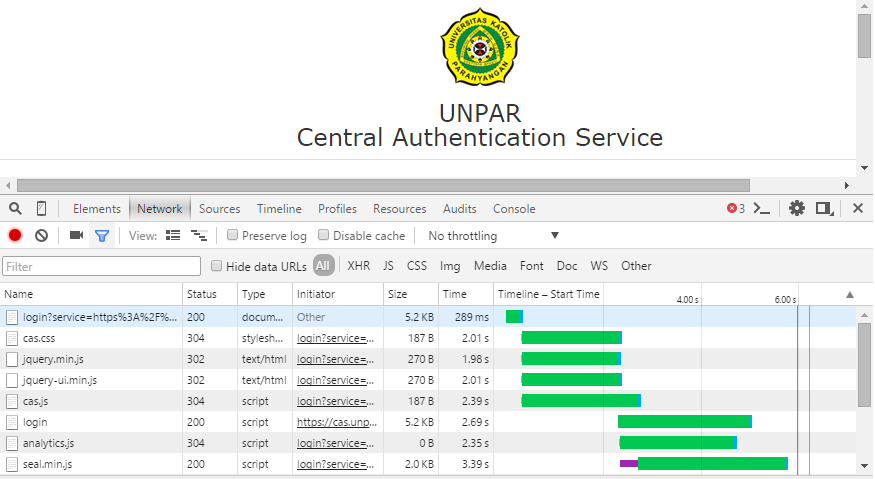
\includegraphics[scale=0.5]{Gambar/chrome-devtools}
	\caption{Chrome DevTools} 
	\label{fig:2_chrome_devtools}
\end{figure}

Pada bagian berikut akan dijelaskan mengenai dua panel dari DevTools.

\textbf{Elements}\\
Panel Elements memungkinkan untuk memperlihatkan informasi yang terstruktur tentang halaman yang sedang dibuka. HTML akan ditampilkan dalam bentuk pohon \textit{Document Object Model} (DOM). DOM adalah sebuah struktur seperti pohon yang dibuat oleh browser untuk menemukan elemen HTML \footnote{\url{http://try.jquery.com/}, diakses 24 September 2015}. Tampilan pohon DOM memperlihatkan struktur DOM dari halaman yang sedang dibuka. Pohon DOM adalah pohon dari node-node yang mewakili setiap elemen HTML seperti \texttt{<body>} dan \texttt{<p>}. 

Pemeriksaan elemen akan memperlihatkan node DOM dan CSS dari elemen yang dipilih pada \textit{browser}. Pemeriksaan elemen dapat dilakukan dengan cara klik kanan pada elemen yang ingin diperiksa kemudian pilih ``Inspect element''. Dengan melakukan pemeriksaan elemen, jendela panel Elements akan muncul. Sebagai contoh pada gambar \ref{fig:2_elements_panel}, saat melakukan ``Inspect element'' pada nama mahasiswa, panel Elements akan muncul dan menunjukkan pohon DOM dari halaman tersebut. Selain itu panel Elements juga menunjukkan CSS selector dari elemen tersebut yaitu \texttt{p.student-name}.

\begin{figure}[H]
	\centering
	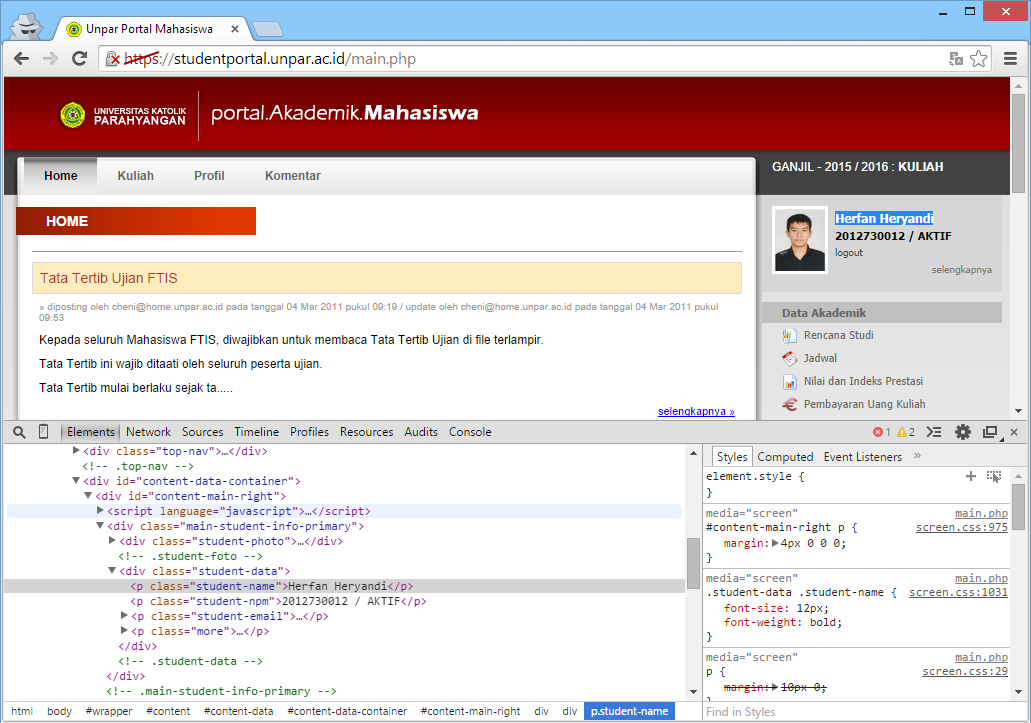
\includegraphics[scale=0.5]{Gambar/elements-panel}
	\caption{Panel Elements} 
	\label{fig:2_elements_panel}
\end{figure}

\textbf{Network}\\
Panel Network secara otomatis merekam semua aktivitas jaringan saat DevTools terbuka. Pertama kali dibuka, panel Network masih kosong. Halaman web harus dimuat ulang untuk mulai merekam aktivitas jaringan atau menunggu adanya aktivitas jaringan pada halaman web. Panel Network akan mencatat sumber daya dari aktivitas jaringan yang terekam. Setiap sumber daya akan ditambahkan ke dalam sebuah baris dalam tabel Network seperti pada gambar \ref{fig:2_network_panel} dengan rincian kolom sebagai berikut:
\begin{itemize}
	\item \textbf{Name dan Path}, nama dan URL dari sumber daya.
	\item \textbf{Method}, metode permintaan HTTP.
	\item \textbf{Status dan Text}, kode status HTTP dan pesan.
	\item \textbf{Domain}, domain dari sumber daya.
	\item \textbf{Type}, tipe sumber daya yang diminta.
	\item \textbf{Cookies}, banyaknya \textit{cookie} yang dikirim dalam permintaan.
	\item \textbf{Size dan Content}, \textit{size} merupakan ukuran dari \textit{header} dan \textit{body} jawaban yang dikirim server sedangkan \textit{content} merupakan ukuran konten sumber daya.
	\item \textbf{Timeline}, alur waktu dari seluruh aktivitas jaringan yang diminta.
\end{itemize}

\begin{figure}[H]
	\centering
	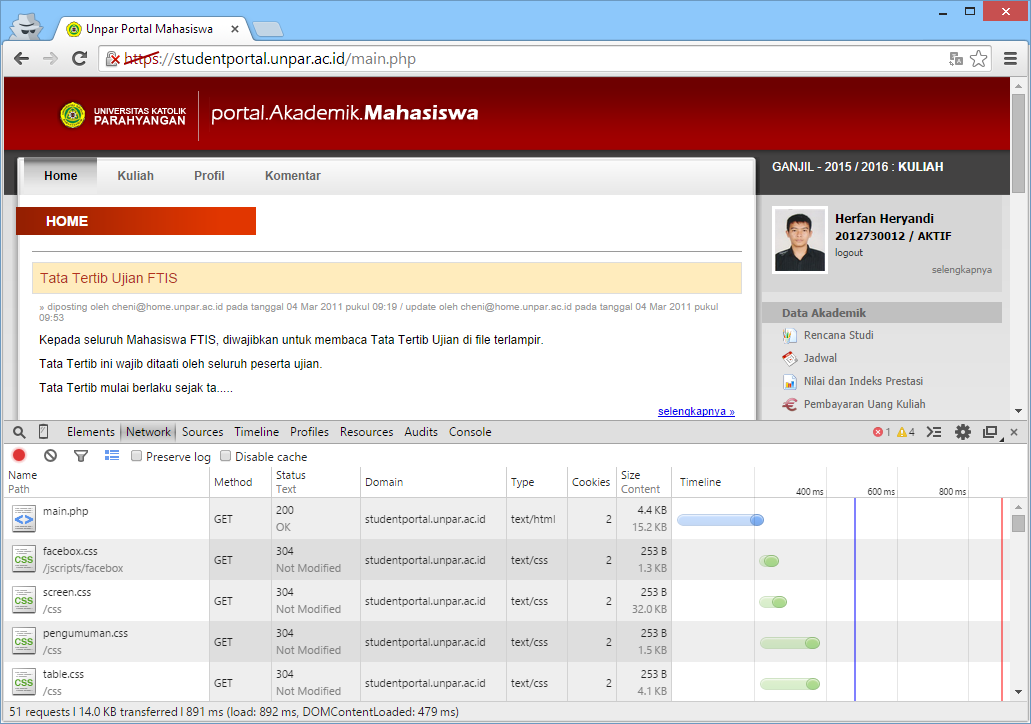
\includegraphics[scale=0.5]{Gambar/network-panel}
	\caption{Panel Network} 
	\label{fig:2_network_panel}
\end{figure}

Ketika nama sumber daya dalam tabel Network diklik, maka akan muncul tautan baru yang berisi rincian tambahan sebagai berikut:
\begin{itemize}
	\item \textbf{Header}\\
	Tautan Header menampilkan \textit{request} URL, \textit{request method}, \textit{status code}, HTTP \textit{response} dan \textit{request header} beserta nilainya, dan \textit{query string parameter}. HTTP header dapat ditampilkan secara terformat atau dalam bentuk sumber dengan mengklik tombol \textit{toggle} ``view parsed''/``view source''. Nilai-nilai parameter dapat ditampilkan dalam bentuk yang sudah didekodekan atau dalam bentuk URL yang dienkode dengan mengklik tombol \textit{toggle} ``view decoded''/``view URL encoded''. Sebagai contoh pada gambar \ref{fig:2_network_get} menampilkan \textit{header} pada metode permintaan GET sedangkan gambar \ref{fig:2_network_post} menampilkan \textit{header} pada metode permintaan POST.
	
\begin{figure}[H]
	\centering
	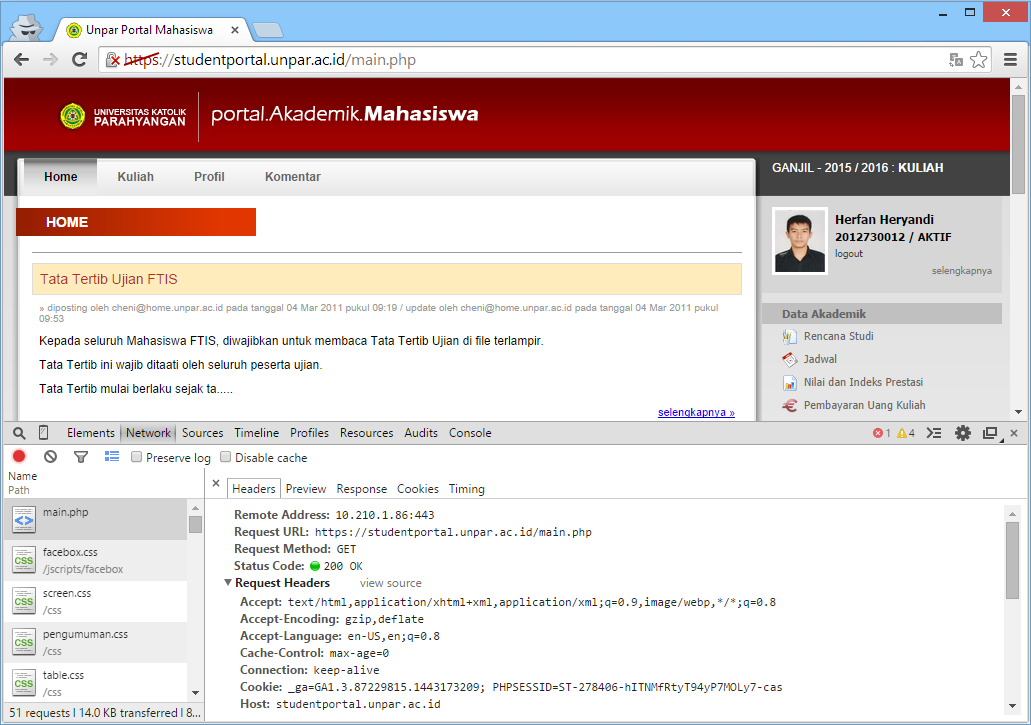
\includegraphics[scale=0.5]{Gambar/network-header}
	\caption{Contoh Tautan Header pada Metode Permintaan GET} 
	\label{fig:2_network_get}
\end{figure}

\begin{figure}[H]
	\centering
	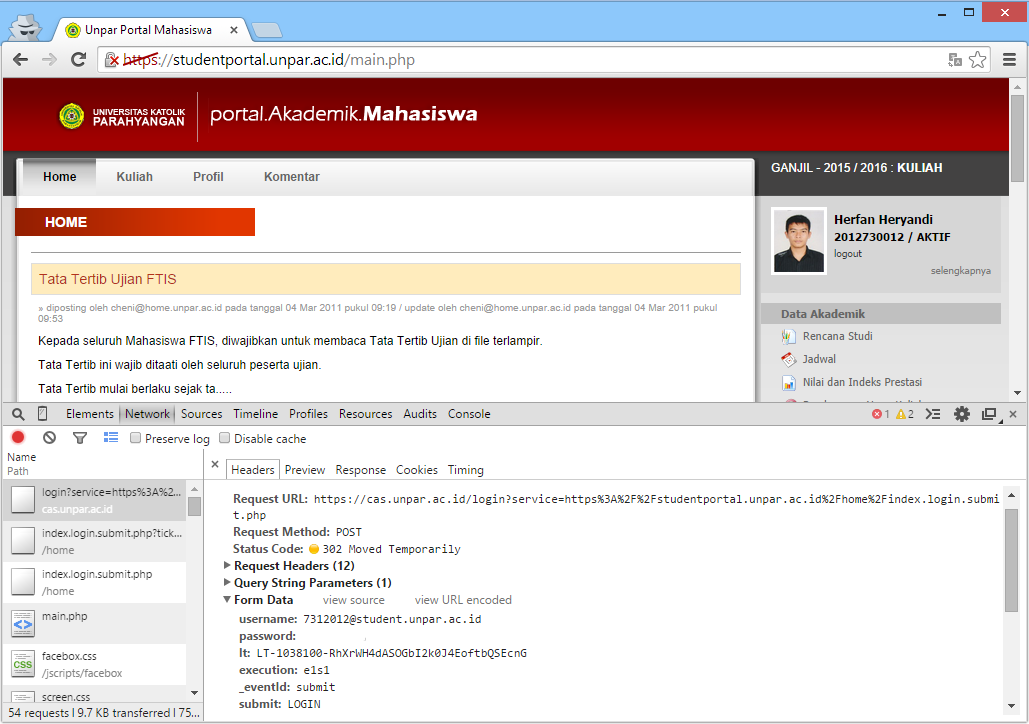
\includegraphics[scale=0.5]{Gambar/network-post}
	\caption{Contoh Tautan Header pada Metode Permintaan POST} 
	\label{fig:2_network_post}
\end{figure}

	\item \textbf{Preview}\\
	Tautan Preview menampilkan \textit{preview} sumber daya jika tersedia. Gambar \ref{fig:2_network_prev_available} menampilkan \textit{preview} yang tersedia pada sumber daya. Jika \textit{preview} tidak tersedia maka akan tampilan akan sama dengan jawaban seperti yang terlihat pada gambar \ref{fig:2_network_prev_notavailable}.
	
\begin{figure}[H]
	\centering
	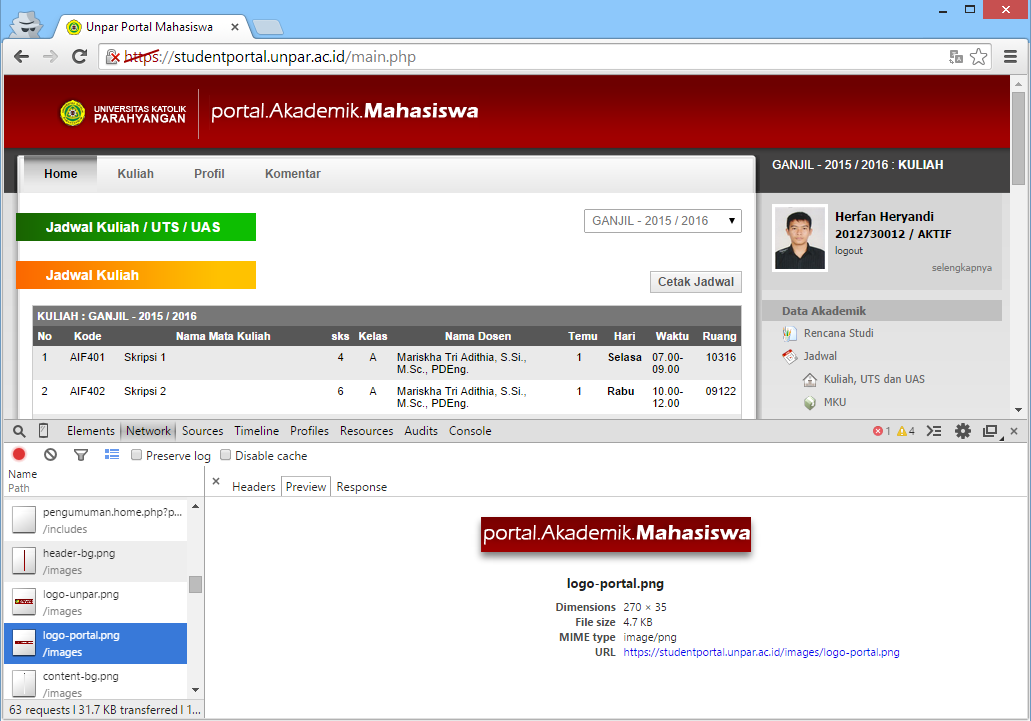
\includegraphics[scale=0.5]{Gambar/network-preview-available}
	\caption{Contoh \textit{Preview} yang Tersedia} 
	\label{fig:2_network_prev_available}
\end{figure}

\begin{figure}[H]
	\centering
	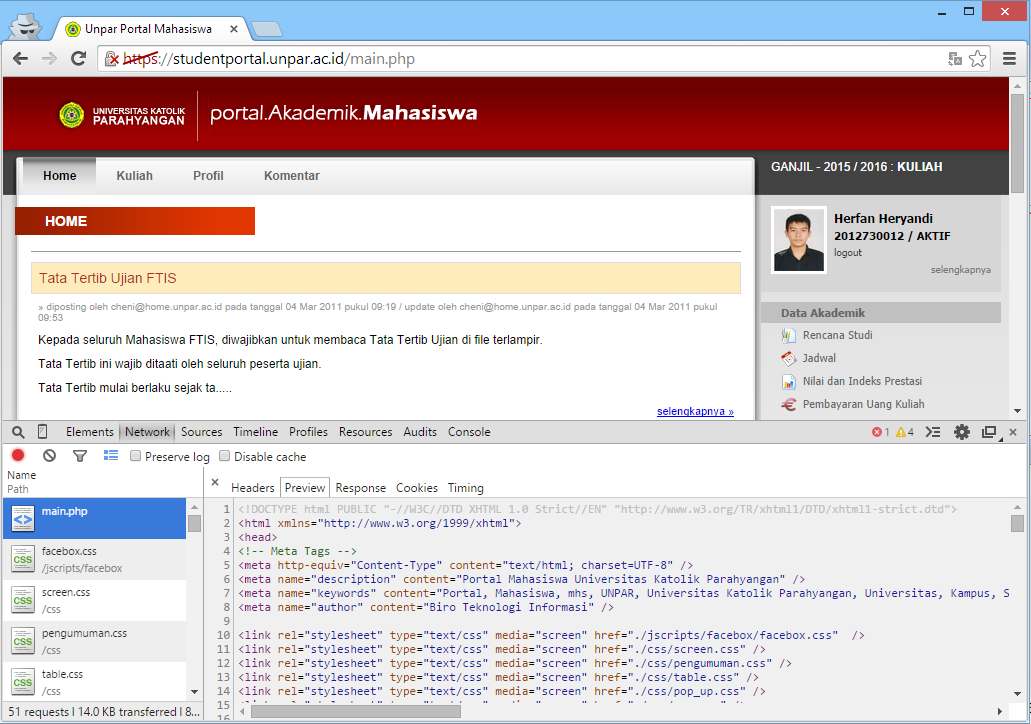
\includegraphics[scale=0.5]{Gambar/network-preview-notAvailable}
	\caption{Contoh \textit{Preview} yang Tidak Tersedia} 
	\label{fig:2_network_prev_notavailable}
\end{figure}

	\item \textbf{Response}\\
	Tautan Response berisi konten symber daya yang tidak terformat. Sebagai contoh pada gambar \ref{fig:2_network_response} menampilkan Tautan Response dari sumber daya \texttt{main.php}.
\begin{figure}[H]
	\centering
	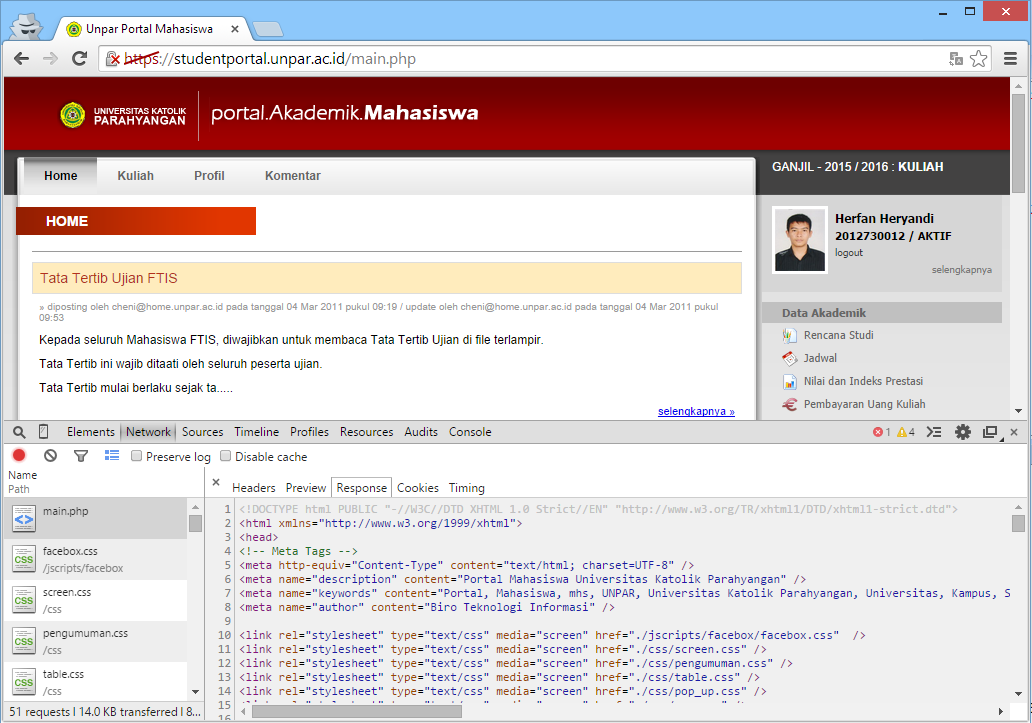
\includegraphics[scale=0.5]{Gambar/network-response}
	\caption{Contoh Tautan Response} 
	\label{fig:2_network_response}
\end{figure}

	\item \textbf{Cookies}\\
	Tautan Cookies menampilkan sebuah tabel yang terdiri dari seluruh \textit{cookie} yang ditransmisikan dalam \textit{header} permintaan dan jawaban HTTP. Contoh dari tabel \textit{cookie} dapat dilihat pada gambar \ref{fig:2_network_cookies} dengan rincian kolom sebagai berikut:
	\begin{itemize}
		\item \textbf{Name}, nama \textit{cookie}
		\item \textbf{Value}, nilai \textit{cookie}
		\item \textbf{Domain}, domain yang memiliki \textit{cookie}
		\item \textbf{Path}, URL asal \textit{cookie}
		\item \textbf{Expires/Max-Age}, batas akhir nilai \textit{cookie}
		\item \textbf{Size}, ukuran \textit{cookie} dalam byte
		\item \textbf{HTTP}, menunjukkan bahwa \textit{cookie} harus ditetapkan oleh browser dalam permintaan HTTP, dan tidak dapat diakses dengan JavaScript
		\item \textbf{Secure}, menunjukkan bahwa \textit{cookie} harus dikirim melalui koneksi yang aman
	\end{itemize}
	
\begin{figure}[H]
	\centering
	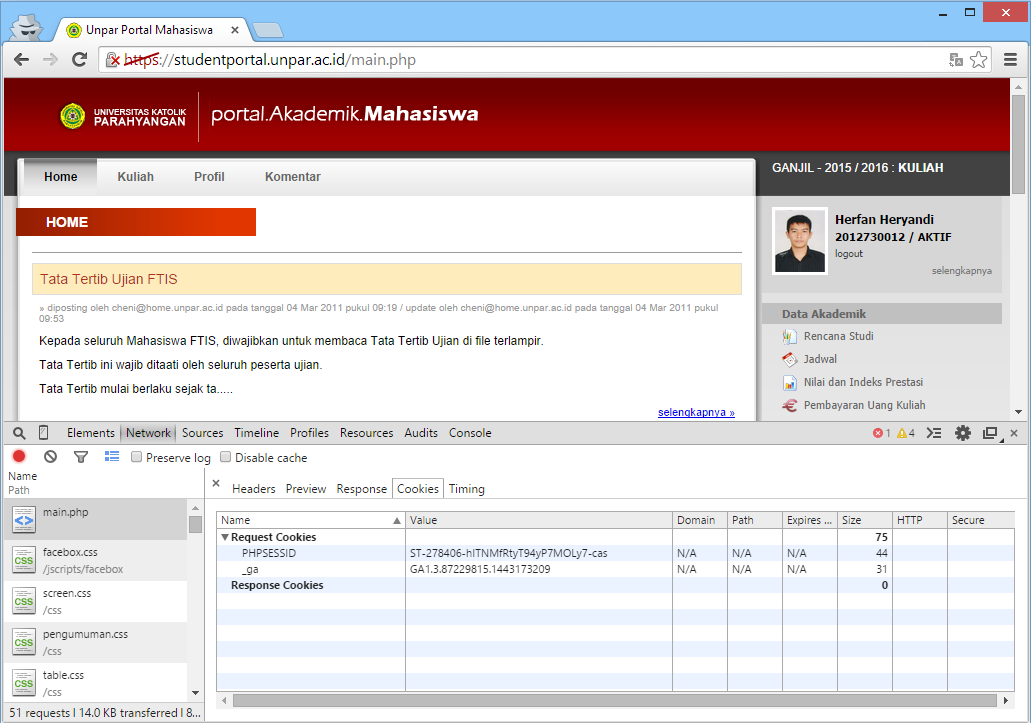
\includegraphics[scale=0.5]{Gambar/network-cookies}
	\caption{Contoh Tabel pada Tautan Cookie} 
	\label{fig:2_network_cookies}
\end{figure}

\end{itemize}

\item\textbf{Play Framework}

Play Framework\cite{Leroux:2014} merupakan sebuah web \textit{framework} berbasis bahasa Java dan Scala. Play Framework juga menggunakan \textit{design pattern} Model-View-Controller (MVC) di mana \textit{model} dan \textit{controller} menggunakan bahasa Java sedangkan \textit{view} menggunakan bahasa Scala dan HTML. Struktur aplikasi Play Framework dapat dilihat pada gambar \ref{fig:2_play_dir}.
\begin{figure}[H]
	\centering
	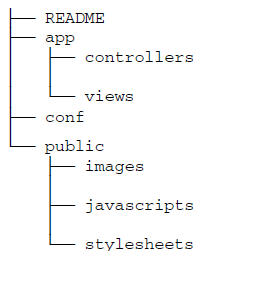
\includegraphics[scale=0.5]{Gambar/play-dir}
	\caption{Struktur Aplikasi Play Framework} 
	\label{fig:2_play_dir}
\end{figure}

Dalam direktori \texttt{conf}, terdapat file \texttt{routes}. Melalui \texttt{routes}, rute aplikasi dapat ditentukan dengan memetakan URL ke kode aplikasi. Setiap \texttt{route} memiliki tiga bagian yaitu HTTP \textit{method}, URL \textit{path}, dan \textit{action method}.  HTTP \textit{method} merupakan metode pengiriman HTTP. URL \textit{path} merupakan URL untuk mengakses halaman. \textit{Action method} merupakan \textit{method} yang menangani permintaan metode pengiriman HTTP. Sebagai contoh pada gambar \ref{fig:2_routes_example}, setiap permintaan GET pada URL \texttt{/list} akan ditangani oleh \textit{method} \texttt{list}() milik kelas \texttt{Products} yang terdapat pada \textit{package} \texttt{controllers}.

\begin{figure}[H]
	\centering
	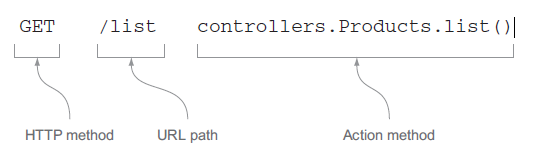
\includegraphics[scale=0.5]{Gambar/contoh-routes}
	\caption{Contoh Komponen \texttt{Route}\cite{Leroux:2014}} 
	\label{fig:2_routes_example}
\end{figure}

Direktori \texttt{app} merupakan sumber dari kode program seperti file Java dan \textit{view}. Saat pertama kali proyek Play Framework dibuat, direktori \texttt{app} berisi file-file seperti pada gambar \ref{fig:2_app_dir}. Dalam folder \texttt{controllers}, terdapat file \texttt{Application.java} yang berisi kode Java untuk menghasilkan halaman web. Kelas yang menangani permintaan HTTP dan mengembalikan hasil HTTP disebut kelas \textit{controller}. Kelas \textit{controller} merupakan kelas yang memiliki \textit{action method}. Setiap \textit{action method} memiliki tipe kembalian \textit{Result} yang merepresentasikan \textit{view}. \textit{Action method} kan berhubungan dengan \textit{view} setelah didefinisikan di \texttt{routes}. \textit{Controller} dapat mengirimkan \textit{parameter} pada \textit{view} melalui kembalian dari \textit{action method}. Sebagai contoh pada gambar \ref{fig:2_exam_ctrl}, \textit{method} \texttt{home()} mengembalikan \textit{view} \texttt{home} yang berada pada \textit{package} \texttt{views} dengan mengirim \textit{parameter} ``nama''.

\begin{figure}[H]
	\centering
	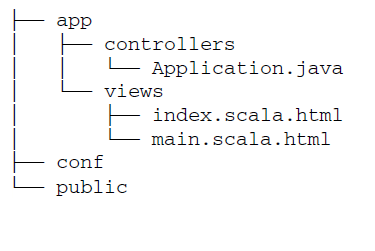
\includegraphics[scale=0.5]{Gambar/app-dir}
	\caption{Direktori \texttt{app} yang Dibangkitkan Play Framework\cite{Leroux:2014}} 
	\label{fig:2_app_dir}
\end{figure}

\begin{figure}[H]
	\centering
	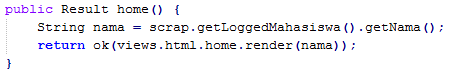
\includegraphics[scale=0.75]{Gambar/example-controller}
	\caption{Contoh \textit{Method} pada Kelas \textit{Controller}} 
	\label{fig:2_exam_ctrl}
\end{figure}

Dalam folder \texttt{views} terdapat dua file yaitu \texttt{index.scala.html} dan \texttt{main.scala.html} yang berfungsi untuk mendefinisikan halaman HTML. Setiap konten yang dihasilkan pada server dan dikirim ke klien dalam \textit{body} HTTP, seperti halaman HTML, disebut \textit{view}. \textit{View} dapat menerima \textit{parameter} dari \textit{controller} menggunakan bahasa Scala. Sebagai contoh pada gambar \ref{fig:2_exam_view}, pada baris pertama ``message'' mendefinisikan nama \textit{parameter} yang diterima dengan tipe \textit{String}. Tipe yang diterima \textit{view} harus sama dengan tipe yang dikirim \textit{controller} begitu pula banyak \textit{parameter}-nya. Baris ke-10 menampilkan ``message'' pada halaman HTML. Tanda ``@'' menandakan penggunaan bahasa Scala pada \textit{view}. Folder-folder yang terdapat dalam direktori \texttt{app} akan menjadi \textit{package} dalam kode Java.

\begin{figure}[H]
	\centering
	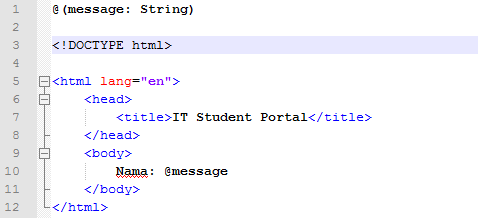
\includegraphics[scale=0.75]{Gambar/example-view}
	\caption{Penerimaan \textit{Parameter} pada \textit{View}} 
	\label{fig:2_exam_view}
\end{figure}

Direktori \texttt{public} berisi sumber yang dapat diakses secara langsung sebagai aset publik. Biasanya aset publik mendukung file selain aplikasi yang dibuat seperti gambar, \textit{stylesheet}, Javascript, dan halaman HTML statis. Aset publik tidak dihasilkan oleh aplikasi melainkan diatur secara langsung oleh pembuat program.

Dalam Play Framework, objek yang disimpan pada \textit{session} memiliki masa hidup yaitu selama \textit{browser} dibuka. \textit{Session} tidak disimpan di server melainkan ditambahkan ke setiap permintaan HTTP berikutnya menggunakan mekanisme \textit{cookie}. Ukuran data \textit{session} sangat terbatas yaitu hingga 4 KB sehingga hanya dapat menyimpan \textit{String}. Pada controller, \textit{session} dapat disimpan dengan \textit{method}:
	\begin{itemize}
			\item \textbf{public static void session(String key, String value)} \\
				\textbf{Parameter:}
				\begin{itemize}
					\item \textbf{key} kunci \textit{session}.
					\item \textbf{value} nilai \textit{session}.
				\end{itemize}
	\end{itemize}
 Sedangkan nilai \textit{session} dapat diperoleh menggunakan \textit{method}: 
\begin{itemize}
			\item \textbf{public static String session(String key)} \\
				\textbf{Parameter:}
				\begin{itemize}
					\item \textbf{key} kunci \textit{session}.
				\end{itemize}
				\textbf{Kembalian:} nilai \textit{session}.
	\end{itemize}


\item\textbf{SIA Models}

SIA Models merupakan kelas-kelas dalam bahasa Java yang merepresentasikan Sistem Informasi Akademik UNPAR\cite{siamodels}. Kelas-kelas yang dimiliki SIA Models terbagi ke dalam tiga package antara lain:

\begin{enumerate}
	\item \textit{Package} \texttt{id.ac.unpar.siamodels}\\
	\textit{Package} ini memiliki kelas-kelas sebagai berikut:
	\begin{enumerate}
		\item Mahasiswa\\
		Kelas ini merepresentasikan mahasiswa. \textit{Method-method} yang dimiliki kelas ini adalah sebagai berikut:
		\begin{itemize}
			\item \textbf{public Mahasiswa(String npm)}\\
			Merupakan \textit{constructor} dari kelas Mahasiswa.\\
			\textbf{Parameter:}
			\begin{itemize}
				\item \textbf{npm} nomor pokok mahasiswa.
			\end{itemize}
			
			\item \textbf{public String getNama()}\\
				Berfungsi untuk mendapatkan nama mahasiswa.\\
				\textbf{Kembalian:} nama mahasiswa.

			\item \textbf{public void setNama(String nama)}\\
				Berfungsi untuk mengubah nama mahasiswa.\\
				\textbf{Parameter:}
				\begin{itemize}
					\item \textbf{nama} nama mahasiswa.
				\end{itemize}
		
			\item \textbf{public String getNpm()}\\
				Berfungsi untuk mendapatkan nomor pokok mahasiswa.\\
				\textbf{Kembalian:} nomor pokok mahasiswa.
			
			\item \textbf{public String getEmailAddress()}\\
				Berfungsi untuk mendapatkan \textit{email} mahasiswa.\\
				\textbf{Kembalian:} \textit{email} mahasiswa.
			
			\item \textbf{public List<Nilai> getRiwayatNilai()}\\
				Berfungsi untuk mendapatkan riwayat nilai mahasiswa.\\
				\textbf{Kembalian:} riwayat nilai mahasiswa dalam List.
				
			\item \textbf{public double calculateIPKLulus()}\\
				Menghitung IPK mahasiswa sampai saat ini, dengan aturan kuliah yang tidak lulus tidak dihitung dan jika pengambilan beberapa kali, diambil nilai terbaik. Sebelum memanggil \textit{method} ini, \texttt{getRiwayatNilai()} harus sudah mengandung nilai per mata kuliah.\\
				\textbf{Kembalian:} IPK lulus.
				
			\item \textbf{public double calculateIPS()}\\
				Menghitung IPS semester terakhir sampai saat ini, dengan aturan kuliah yang tidak lulus dihitung. Sebelum memanggil \textit{method} ini, \texttt{getRiwayatNilai()} harus sudah mengandung nilai per mata kuliah.\\
				\textbf{Kembalian:}  nilai IPS sampai saat ini.
				
			\item \textbf{public int calculateSKSLulus()}\\
				Menghitung jumlah SKS lulus mahasiswa saat ini. Sebelum memanggil \textit{method} ini, \texttt{getRiwayatNilai()} harus sudah mengandung nilai per mata kuliah.\\
				\textbf{Kembalian:} SKS lulus.
				
			\item \textbf{public boolean hasLulusKuliah(String kodeMataKuliah)}\\
				Memeriksa apakah mahasiswa ini sudah lulus mata kuliah tertentu. Sebelum memanggil \textit{method} ini, \texttt{getRiwayatNilai()} harus sudah mengandung nilai per mata kuliah.\\
				\textbf{Parameter:}
				\begin{itemize}
					\item \textbf{kodeMataKuliah} kode mata kuliah yang ingin diperiksa kelulusannya.
				\end{itemize}
				\textbf{Kembalian:} \texttt{true} jika sudah pernah mengambil dan lulus, \texttt{false} jika belum.
				
			\item \textbf{public boolean hasTempuhKuliah(String kodeMataKuliah)}\\
				Memeriksa apakah mahasiswa ini sudah pernah menempuh mata kuliah tertentu. Sebelum memanggil \textit{method} ini, \texttt{getRiwayatNilai()} harus sudah mengandung nilai per mata kuliah.\\
				\textbf{Parameter:}
				\begin{itemize}
					\item \textbf{kodeMataKuliah} kode mata kuliah yang ingin diperiksa kelulusannya.
				\end{itemize}
				\textbf{Kembalian:} \texttt{true} jika sudah pernah mengambil, \texttt{false} jika belum.
			
			\item \textbf{public int getTahunAngkatan()}\\
				Mendapatkan tahun angkatan mahasiswa ini berdasarkan NPM-nya.\\
				\textbf{Kembalian:} tahun angkatan.
			\end{itemize}
		
		\item Nilai\\
		Kelas ini merepresentasikan nilai yang ada pada riwayat nilai mahasiswa. \textit{Method-method} yang dimiliki kelas ini adalah sebagai berikut:
		\begin{itemize}
			\item \textbf{public Nilai(int tahunAjaran, int semester, MataKuliah mataKuliah, Character kelas, Double nilaiART, Double nilaiUTS, Double nilaiUAS, Character nilaiAkhir)}\\
				Merupakan \textit{constructor} dari kelas Nilai.\\
				\textbf{Parameter:}
				\begin{itemize}
					\item \textbf{tahunAjaran} tahun ajaran kuliah ini diambil.
					\item \textbf{semester} semester kuliah ini diambil.
					\item \textbf{mataKuliah} mata kuliah yang diambil.
					\item \textbf{kelas} kelas kuliah.
					\item \textbf{nilaiART} nilai ART.
					\item \textbf{nilaiUTS} nilai UTS.
					\item \textbf{nilaiUAS} nilai UAS.
					\item \textbf{nilaiAkhir} nilai akhir.
				\end{itemize}
				
			\item \textbf{public MataKuliah getMataKuliah()}\\
				Mendapatkan mata kuliah yang diambil.\\
				\textbf{Kembalian:} mata kuliah.
				
			\item \textbf{public Character getKelas()}\\
				Mendapatkan kelas kuliah.\\
				\textbf{Kembalian:} kelas kuliah.
				
			\item \textbf{public Double getNilaiART()}\\
				Mendapatkan nilai ART.\\
				\textbf{Kembalian:} nilai ART.
				
			\item \textbf{public Double getNilaiUTS()}\\
				Mendapatkan nilai UTS.\\
				\textbf{Kembalian:} nilai UTS.
				
			\item \textbf{public Double getNilaiUAS()}\\
				Mendapatkan nilai UAS.\\
				\textbf{Kembalian:} nilai UAS.
				
			\item \textbf{public Double getNilaikhir()}\\
				Mendapatkan nilai akhir dalam bentuk angka.\\
				\textbf{Kembalian:} nilai akhir dalam huruf atau \texttt{null} jika tidak ada.
			
			\item \textbf{public Double getAngkaAkhir()}\\
				Mengembalikan nilai akhir dalam bentuk huruf (A, B, C, D, ...).\\
				\textbf{Kembalian:} nilai akhir dalam angka, atau \texttt{null} jika \texttt{getNilaiAkhir()} mengembalikan \texttt{null}.
			
			\item \textbf{public int getTahunAjaran()}\\
				Mendapatkan tahun ajaran saat pengambilan mata kuliah.\\
				\textbf{Kembalian:} tahun ajaran saat pengambilan mata kuliah.
			
			\item \textbf{public int getTahunSemester()}\\
				Mendapatkan semester pengambilan mata kuliah.\\
				\textbf{Kembalian:} semester pengambilan mata kuliah.	
		\end{itemize}
		
		\item ChronologicalComparator\\
		Pembanding antara satu nilai dengan nilai lainnya, secara kronologis waktu pengambilan. \textit{Method} yang dimiliki kelas ini adalah sebagai berikut:
		
		\begin{itemize}
			\item \textbf{public int compare(Nilai o1, Nilai o2) } \\
			Berfungsi untuk membandingkan nilai. \\
			\textbf{Parameter:}
			\begin{itemize}
				\item \textbf{o1} nilai pertama yang akan dibandingkan.
				\item \textbf{o2} nilai kedua yang akan dibandingkan.
			\end{itemize}
			\textbf{Kembalian:} hasil perbandingan.
		\end{itemize}
		
		\item MataKuliah\\
		Kelas ini merepresentasikan sebuah mata kuliah. \textit{Method-method} yang dimiliki kelas ini adalah sebagai berikut:
		\begin{itemize}
			\item \textbf{protected MataKuliah(String kode, int sks, String nama)} \\
			Merupakan \textit{constructor} dari kelas MataKuliah.\\
			\textbf{Parameter:}
			\begin{itemize}
				\item \textbf{kode} kode mata kuliah.
				\item \textbf{sks} bobot SKS mata kuliah.
				\item \textbf{nama} nama mata kuliah.
			\end{itemize}
			
			\item \textbf{public String getKode()}\\
				Mendapatkan kode mata kuliah.\\
				\textbf{Kembalian:} kode mata kuliah.
				
			\item \textbf{public int getSKS()}\\
				Mendapatkan bobot SKS mata kuliah.\\
				\textbf{Kembalian:} bobot SKS mata kuliah.
				
			\item \textbf{public String getNama()}\\
				Mendapatkan nama mata kuliah.\\
				\textbf{Kembalian:} nama mata kuliah.
				
			\item \textbf{public static MataKuliah createMataKuliah(String kode, int sks, String nama)} \\
			Mendapatkan atau membuat mata kuliah baru.\\
			\textbf{Parameter:}
			\begin{itemize}
				\item \textbf{kode} kode mata kuliah.
				\item \textbf{sks} bobot SKS mata kuliah.
				\item \textbf{nama} nama mata kuliah.
			\end{itemize}
			\textbf{Kembalian:} objek mata kuliah.
			
			\item \textbf{public static MataKuliah getMataKuliah(String kode)}\\
				Mendapatkan mata kuliah.\\
				\textbf{Parameter:}
				\begin{itemize}
					\item \textbf{kode} kode mata kuliah.
				\end{itemize}
				\textbf{Kembalian:} mata kuliah sesuai kode.	
		\end{itemize}
		
		\item Semester\\
		Kelas ini menyimpan konstanta untuk semester-semester di UNPAR. Nilai konstanta harus sesuai urutan kronologis dalam satu tahun ajaran. \textit{Method} yang dimiliki kelas ini adalah sebagai berikut:
		\begin{itemize}
			\item \textbf{public static final int fromString(String text)} \\
			Berfungsi untuk mengubah semester dari bentuk teks ke konstanta. \\
			\textbf{Parameter:}
			\begin{itemize}
				\item \textbf{text} semester dalam bentuk teks (GANJIL, GENAP, PENDEK).
			\end{itemize}
			\textbf{Kembalian:} konstanta semester.
		\end{itemize}
	\end{enumerate}
	
	\item \textit{Package} \texttt{id.ac.unpar.siamodels.matakuliah.interfaces}\\
	\textit{Package} ini memiliki beberapa \textit{interface} antara lain:
	\begin{enumerate}
		\item HasPrasyarat\\
		Mendefinisikan kelas-kelas yang memiliki prasyarat, terkustomisasi untuk seorang mahasiswa. \textit{Method} yang dimiliki \textit{interface} ini adalah sebagai berikut: 
		\begin{itemize}
			\item \textbf{public boolean checkPrasyarat(Mahasiswa mahasiswa, List<String> reasonsContainer)} \\
			Memeriksa prasyarat-prasyarat dari kuliah, spesifik untuk mahasiswa yang dituju. Jika ada pesan-pesan khusus, akan ditambahkan pada parameter reasonsContainer.\\
			\textbf{Parameter:}
			\begin{itemize}
				\item \textbf{mahasiswa} prasyarat kuliah akan diperiksa spesifik pada mahasiswa ini.
				\item \textbf{reasonsContainer} jika pesan-pesan terkait prasyarat akan ditambahkan di sini.
			\end{itemize}
			\textbf{Kembalian:} \texttt{true} jika seluruh prasyarat dipenuhi, \texttt{false} jika tidak.
		\end{itemize}
		
		\item Pilihan\\
		Mendefinisikan kelas-kelas yang merupakan mata kuliah pilihan.
		\item PilihanWajib\\
		Mendefinisikan kelas-kelas yang merupakan mata kuliah pilihan wajib.
		\item Wajib\\
		Mendefinisikan kelas-kelas yang merupakan mata kuliah wajib.
	\end{enumerate}
	
	\item \textit{Package} \texttt{id.ac.unpar.siamodels.matakuliah}\\
	\textit{Package} ini berisi kelas-kelas yang merepresentasikan mata kuliah yang terdapat pada Program Studi Teknik Informatika UNPAR. Rincian dari kelas-kelas pada package ini dapat dilihat pada tabel \ref{tab:2_kelas_matakuliah}.

\begin{table}[H]
	\centering
    \begin{tabular}{|p{2.5cm}|p{4.5cm}|p{2.5cm}|p{4.5cm}|}
		\hline
		Kelas & \textit{Implements} & Kelas & \textit{Implements}\\
		\hline
    AIF101  & - &    AIF342  & HasPrasyarat               \\
    AIF102  & HasPrasyarat, Wajib        &    AIF344  & HasPrasyarat               \\
    AIF103  & -                          &    AIF360  & HasPrasyarat               \\
    AIF105  & -                          &    AIF362  & HasPrasyarat, Pilihan      \\
    AIF200  & -                          &    AIF401  & HasPrasyarat, Wajib        \\
    AIF201  & HasPrasyarat, Wajib        &    AIF402  & HasPrasyarat, Wajib        \\
    AIF202  & HasPrasyarat, Wajib        &    AIF403  & -                          \\
    AIF203  & HasPrasyarat, Wajib        &    AIF405  & HasPrasyarat, Wajib        \\
    AIF204  & HasPrasyarat               &    AIF438  & HasPrasyarat, Pilihan      \\
    AIF205  & HasPrasyarat, Wajib        &    AIF441  & -                          \\
    AIF206  & HasPrasyarat               &    AIF445  & HasPrasyarat               \\
    AIF208  & HasPrasyarat               &    AIF453  & HasPrasyarat, Pilihan      \\
    AIF301  & HasPrasyarat, Wajib        &    AIF456  & -                          \\
    AIF302  & HasPrasyarat, Wajib        &    AIF457  & HasPrasyarat, Pilihan      \\
    AIF303  & HasPrasyarat, Wajib        &    AIF458  & HasPrasyarat               \\
    AIF304  & HasPrasyarat               &    AIF461  & HasPrasyarat               \\
    AIF305  & HasPrasyarat, Wajib        &    AIF462  & -                          \\
    AIF306  & HasPrasyarat               &    AIF469  & HasPrasyarat, Pilihan      \\
    AIF311  & HasPrasyarat, PilihanWajib &    APS402  & HasPrasyarat, Wajib        \\
    AIF312  & HasPrasyarat               &    MKU001  & -                          \\
    AIF314  & HasPrasyarat, PilihanWajib &    MKU002  & -                          \\
    AIF315  & HasPrasyarat, PilihanWajib &    MKU003  & -                          \\
    AIF316  & HasPrasyarat               &    MKU004  & -                          \\
    AIF317  & HasPrasyarat, PilihanWajib &    MKU008  & -                          \\
    AIF318  & HasPrasyarat               &    MKU009  & -                          \\
    AIF332  & HasPrasyarat               &    MKU010  & -                          \\
    AIF336  & -                          &    MKU011  & -                          \\
    AIF339  & HasPrasyarat               &    MKU012  & -                          \\
    AIF341  & -                          &            &           				   \\
		\hline
    \end{tabular}
		\caption{Tabel Rincian Kelas pada \textit{Package} \texttt{id.ac.unpar.siamodels.matakuliah}}
	\label{tab:2_kelas_matakuliah}
\end{table}

\end{enumerate}

\item \textbf{CSS \textit{Selector}}

CSS(\textit{Cascading Style Sheets}) memungkinkan adanya perubahan terhadap teks dari elemen HTML yang sudah didefinisikan\cite{Meyer:2012}. Seperti yang ditampilkan pada gambar \ref{fig:2_selector_ex}, defini CSS memiliki dua komponen yaitu selector dan properti. CSS \textit{selector} digunakan untuk mendefinisikan elemen HTML sedangkan properti mendefinisikan atribut beserta nilai. 
		\begin{figure}[H]
			\centering
			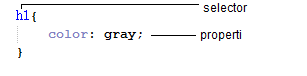
\includegraphics[scale=0.8]{Gambar/selector-ex}
			\caption{Format Penulisan Definisi CSS} 
			\label{fig:2_selector_ex}
		\end{figure}
Beberapa jenis CSS \textit{Selector} antara lain:
\begin{enumerate}
	\item \textit{\textbf{Element Selector}}, memilih \textit{tag} html.\\
		Contoh: \texttt{h1}\\
		Keterangan: \textit{selector} mendefinisikan elemen h1.
	\item \textit{\textbf{Grouping Selector}}, memilih beberapa \textit{selector} sekaligus. Setiap \textit{selector} dipisahkan dengan ``,''.\\
		Contoh: \texttt{h1, h2, p}\\
		Keterangan: \textit{selector} mendefinisikan elemen h1, h2, dan p.
	\item \textit{\textbf{Universal Selector}}, memilih seluruh elemen. \textit{Selector} ditampilkan sebagai ``*''.\\
		Contoh: \texttt{*}\\
		Keterangan: \textit{selector} mendefinisikan seluruh elemen.
	\item \textit{\textbf{Class Selector}}, memilih kelas elemen. \textit{Selector} ditampilkan sebagai ``.'' kemudian diikuti nama kelas elemen.\\
		Contoh: \texttt{.top}\\
		Keterangan: \textit{selector} mendefinisikan elemen dengan kelas ``top''.
	\item \textit{\textbf{ID Selector}}, memilih ID elemen. \textit{Selector} ditampilkan sebagai ``\#'' kemudian diikuti ID elemen.\\
		Contoh: \texttt{\#top}\\
		Keterangan: \textit{selector} mendefinisikan elemen dengan ID ``top''. 
	\item \textit{\textbf{Attribute Selector}}, akan dijelaskan dua \textit{attribute selector} yaitu:
		\begin{itemize}
			\item \textit{\textbf{Simple Attribute}}, memilih atribut elemen. \textit{Selector} ditampilkan sebagai nama atribut kemudian diapit dengan kurung siku.
			Contoh: \texttt{[name]}\\
			Keterangan: \textit{selector} mendefinisikan elemen dengan atribut ``name''. 
			
			\item \textit{\textbf{Exact Value Attribute}}, memilih atribut elemen dengan nilai tertentu. \textit{Selector} ditampilkan sebagai definisi atribut kemudian diapit dengan kurung siku.
			Contoh: \texttt{[name=Joe]}\\
			Keterangan: \textit{selector} mendefinisikan elemen dengan atribut ``name'' yang memiliki nilai ``Joe''. 
		\end{itemize}
		
	\item \textit{\textbf{Descendant Selector}}, memilih \textit{child} elemen yang merupakan keturunan \textit{parent} tertentu. \textit{Selector} ditampilkan dengan mendefinisikan parent kemudian diikuti oleh child dipisahkan dengan spasi.\\
			Contoh: \texttt{p .top}\\
			Keterangan: \textit{selector} mendefinisikan elemen dengan kelas ``top'' yang merupakan \textit{child} dari elemen p. 
\end{enumerate}		

\end{enumerate}


		
		%NOMOR 2%
		\item Melakukan wawancara kepada mahasiswa Program Studi Teknik Informatika untuk mendapatkan informasi
penggunaan Portal Akademik Mahasiswa dan fitur-fitur yang diinginkan.\\
		{\bf status :} Ada sejak rencana kerja skripsi.\\
		{\bf hasil :}  \\
		Dalam menganalisis kebutuhan IT Student Portal, penulis melakukan wawancara dengan 18 mahasiswa Program Studi Teknik Informatika UNPAR. Kriteria dari 18 mahasiswa tersebut yaitu sembilan mahasiswa angkatan 2012, delapan mahasiswa angkatan 2013, dan satu mahasiswa angkatan 2014. Bukti-bukti wawancara dapat dilihat pada \url{https://github.com/herfanheryandi/Skripsi/tree/master/draft/Interview/}. Setelah melakukan wawancara, penulis memperoleh fitur-fitur yang diinginkan mahasiswa antara lain:
\begin{enumerate}
	\item Prasyarat mata kuliah\\
	Mahasiswa bisa memeriksa prasyarat mata kuliah saat FRS sehingga tidak terjadi kesalahan pengambilan mata kuliah. Prasyarat mata kuliah yang ditampilkan di Portal Akademik Mahasiswa kurang akurat. Selain itu, dari 18 mahasiswa yang diwawancara, hanya ada satu mahasiswa yang mengetahui bahwa Portal Akademik Mahasiswa memiliki fitur prasyarat. Prasyarat mata kuliah untuk Program Studi Teknik Informatika juga tersedia di \url{http://tinyurl.com/lionov}, namun mahasiswa merasa kurang praktis karena harus memeriksa secara manual. Mahasiswa menginginkan agar fitur ini bisa dibuat untuk mempermudah FRS.
	\item Ringkasan data akademik\\
	Ringkasan data akademik menampilkan data mengenai mata kuliah wajib, pilihan, dan pilihan wajib yang sudah lulus, mata kuliah wajib yang belum lulus, dan sisa SKS untuk mencapai kelulusan. Mahasiswa menginginkan fitur ini dibuat untuk membantu mahasiswa dalam mengatur perkuliahannya.
	\item Perubahan IPS dan IPK berdasarkan riwayat nilai\\
	Dalam Portal Akademik Mahasiswa, nilai pertama kali muncul dalam riwayat nilai. Riwayat IP tidak berubah secara otomatis saat seluruh nilai di riwayat nilai sudah muncul. Mahasiswa menginginkan agar IPS dan IPK dapat berubah secara otomatis saat nilai muncul.
	\item Jadwal kuliah yang tersusun\\
	Tampilan jadwal kuliah dalam Portal Akademik Mahasiswa tidak terurut berdasarkan hari seperti pada gambar \ref{fig:3_jadwal_portal} sehingga perlu direkapitulasi lagi. Mahasiswa menginginkan agar tampilan jadwal tersusun dan dalam bentuk seperti gambar \ref{fig:3_jadwal_rekap}.
		\begin{figure}[H]
			\centering
			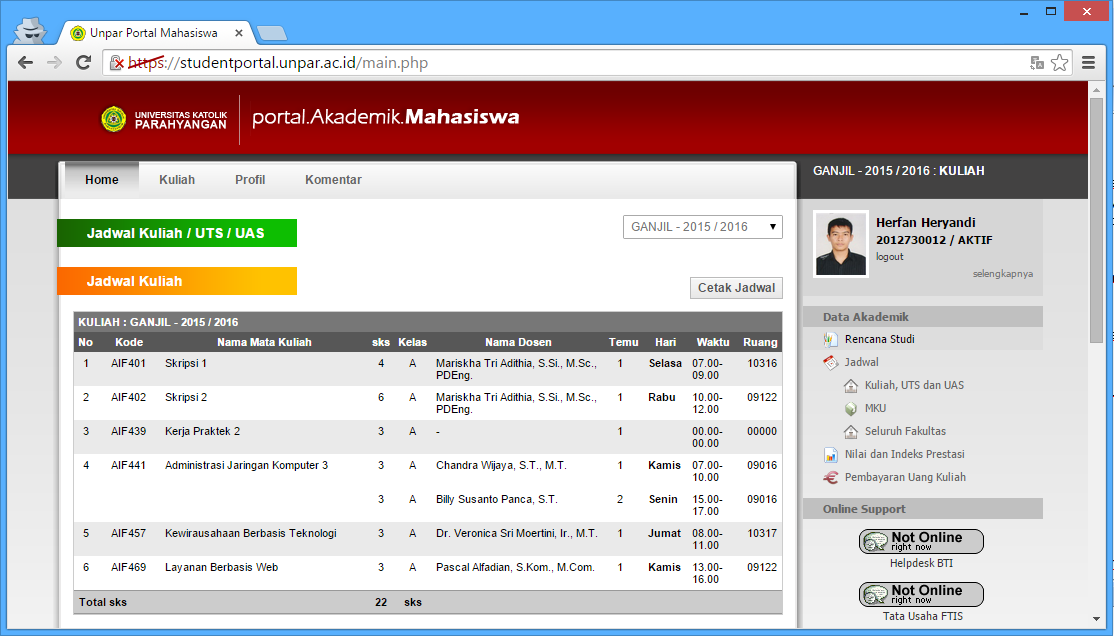
\includegraphics[scale=0.5]{Gambar/jadwal-portal}
			\caption{Tampilan Jadwal pada Portal Akademik Mahasiswa} 
			\label{fig:3_jadwal_portal}
		\end{figure}
		
		\begin{figure}[H]
			\centering
			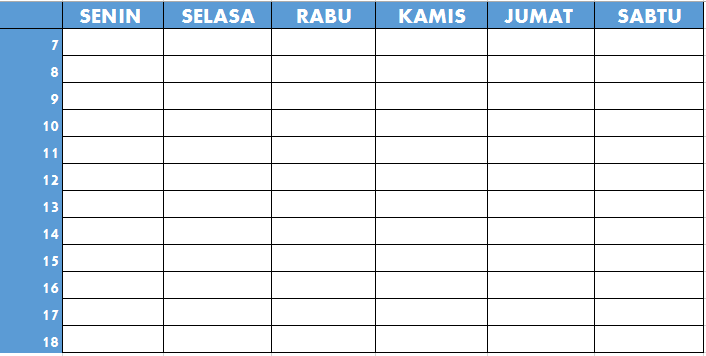
\includegraphics[scale=0.5]{Gambar/jadwal-rekap}
			\caption{Tampilan Jadwal yang Diinginkan Mahasiswa} 
			\label{fig:3_jadwal_rekap}
		\end{figure}
		
	\item Kalender akademik\\
	Kalender akademik merupakan salah satu fitur pada Portal Akademik Mahasiswa namun sekarang fitur tersebut sudah tidak ada lagi. Mahasiswa menginginkan fitur kalender akademik kembali untuk mengetahui tanggal-tanggal penting pada perkuliahan. 
	\item Rincian pembayaran\\
	Tagihan pada Portal Akademik Mahasiswa tidak mencantumkan batas akhir pembayaran dan rincian nominal tagihan. Mahasiswa menginginkan rincian pembayaran agar tidak terlambat membayar uang kuliah dan dapat mengetahui rincian nominal tagihan.
	\item Rincian mata kuliah\\
	Setiap mata kuliah yang dibuka memiliki rincian seperti deskripsi mata kuliah dan jenis mata kuliah yaitu apakah mata kuliah tersebut wajib, pilihan, atau pilihan wajib. Mahasiswa menginginkan fitur ini agar dapat mengetahui mata kuliah apa yang akan dipelajari.
	\item Tampilan situs web sama di sistem operasi manapun\\
	Jika tidak menggunakan sistem operasi Windows seperti Linux dan Mac, saat mengakses Portal Akademik Mahasiswa melalui \url{https://studentportal.unpar.ac.id/}, maka mahasiswa akan diarahkan ke \url{https://m.studentportal.unpar.ac.id/} yaitu Portal Akademik Mahasiswa dengan tampilan \textit{mobile} (Gambar \ref{fig:3_pam_mobile}). Tampilan ini tidak memiliki fitur selengkap Portal Akademik Mahasiswa, hanya memiliki fitur pengumunan kuliah, jadwal kuliah, UTS, dan UAS, nilai, IP, dan tagihan. Selain itu, tampilan \textit{mobile} pada telepon seluler akan terlihat sangat kecil sehingga tidak sulit untuk memilih menu. Mahasiswa menginginkan fitur ini agar IT Student Portal dapat diakses di sistem operasi manapun tanpa perubahan tampilan.
	\begin{figure}[H]
			\centering
			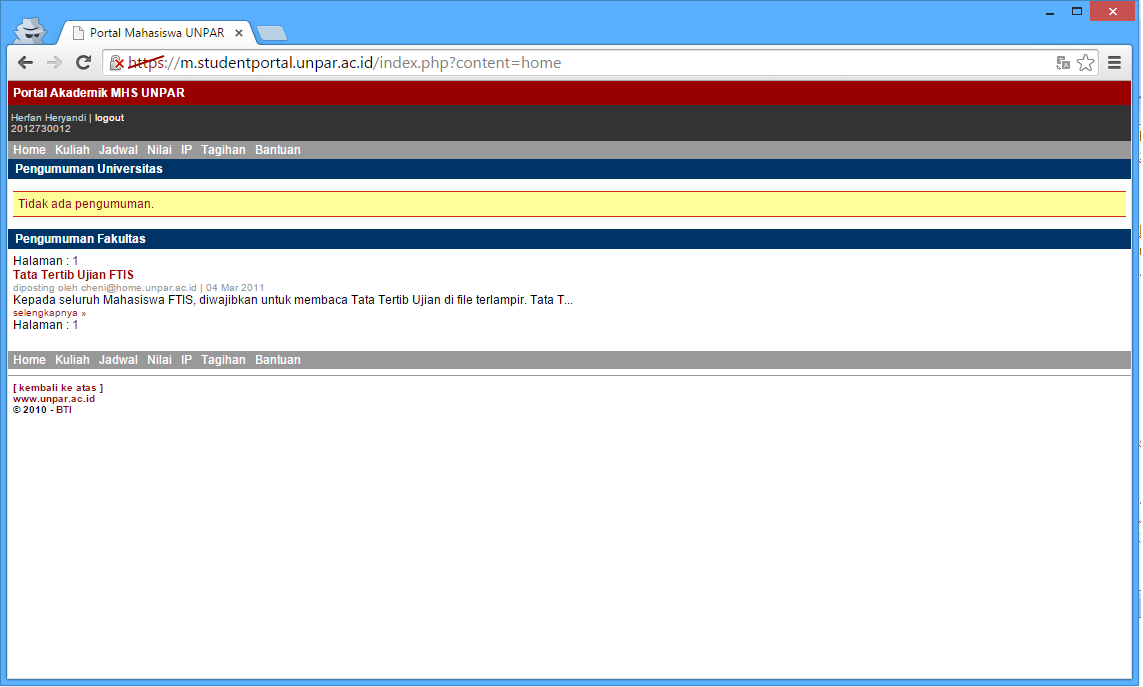
\includegraphics[scale=0.5]{Gambar/pam-mobile}
			\caption{Tampilan \textit{Mobile} Portal Akademik Mahasiswa} 
			\label{fig:3_pam_mobile}
		\end{figure}
	\item Kontak dosen\\
	Kontak dosen berisi informasi email setiap dosen sehingga dapat mempermudah mahasiswa untuk menghubungi dosen. Mahasiswa juga dapat mengirim email secara langsung melalui Portal Akademik Mahasiswa.
	\item Pohon kurikulum\\
	Mahasiswa munginnginkan agar dapat melihat pohon kurikulum Program Studi Teknik Informatika dalam Portal Akademik Mahasiswa.
	\item Pemberitahuan\\
	Mahasiswa menginginkan Portal Akademik Mahasiswa menampilkan pemberitahuan berupa \textit{pop up} mengenai pengumuman terkini.
	\item \textit{Chatting}\\
	Mahasiswa menginginkan agar dapat berkomunikasi dengan sesama pengguna Portal Akademik Mahasiswa melalui \textit{chat}.
	\item Unggah \textit{Curriculum Vitae}
	Mahasiswa menginginkan agar dapat mengunggah data mengenai kegiatan dan keaktifan di universitas agar dapat digunakan oleh perusahaan untuk mencari mahasiswa dengan kriteria tertentu misalnya untuk kepentingan magang dan beasiswa.
\end{enumerate}

Fitur-fitur yang akan dipilih untuk diimplementasikan harus memenuhi kriteria:
\begin{itemize}
	\item Data yang dibutuhkan dapat diambil dari Portal Akademik Mahasiwa
	\item Fitur tidak tersedia di Portal Akademik Mahasiswa
	\item Fitur mendukung fungsi Portal Akademik Mahasiswa sebagai sumber informasi akademik
\end{itemize}

Hasil analisis fitur-fitur yang diinginkan berdasarkan kriteria di atas dan batas waktu pembangunan aplikasi dapat dilihat pada tabel \ref{tab:3_hasil_fitur}.
\begin{table}[H]
	\centering
    \begin{tabular}{|p{4.5cm}|p{2.5cm}|p{8cm}|}
		\hline
		Fitur & Dibuat/Tidak dibuat & Alasan\\
		\hline
		Prasyarat mata kuliah                             & Dibuat       & Prasyarat mata kuliah Program Studi Teknik Informatika sudah tersedia di SIA Models                   \\
		\hline
    Ringkasan data akademik                               & Dibuat       & Data dapat diambil dari Portal Akademik Mahasiswa dan didukung oleh SIA Models                        \\
		\hline
    Perubahan IPS dan IPK berdasarkan riwayat nilai   & Dibuat       &  IPS dan IPK dapat dihitung melalui riwayat nilai yang dapat diperoleh dari Portal Akademik Mahasiswa \\
		\hline
    Jadwal kuliah yang tersusun                       & Dibuat       & Jadwal yang tersusun mempermudah mahasiswa untuk                                                      \\
		\hline
    Kalender akademik                                 & Tidak dibuat & Data tidak bisa diperoleh dari Portal Akademik Mahasiwa                                               \\
		\hline
    Rincian pembayaran                                & Tidak dibuat & Data tidak bisa diperoleh dari Portal Akademik Mahasiwa                                               \\
		\hline
    Rincian mata kuliah                               & Tidak dibuat & Data tidak bisa diperoleh dari Portal Akademik Mahasiwa                                               \\
		\hline
    Tampilan situs web sama di sistem operasi manapun & Dibuat       & Aplikasi yang akan dibuat merupakan situs web yang responsif                                          \\
		\hline
    Kontak dosen                                      & Tidak dibuat & Data tidak bisa diperoleh dari Portal Akademik Mahasiwa                                               \\
		\hline
    Pemberitahuan                                     & Tidak dibuat & Waktu pengerjaan yang terbatas                                                                        \\
		\hline
    \textit{Chatting}                                          & Tidak dibuat & Waktu pengerjaan yang terbatas                                                                        \\
		\hline
    Unggah \textit{Curriculum Vitae}                           & Tidak dibuat & Tidak mendukung Portal Akademik Mahasiswa sebagai sumber informasi akademik                           \\
		\hline
		\end{tabular}
		\caption{Tabel Hasil Analisis Kebutuhan IT Student Portal}
	\label{tab:3_hasil_fitur}
\end{table}
		
		%NOMOR 3%
		\item Menganalisis Portal Akademik Mahasiswa dan Perancangan IT Student Portal.\\
		{\bf status :} Ada sejak rencana kerja skripsi, kecuali Analisis Perancangan IT Student Portal.\\
		{\bf hasil :} \\
		\begin{enumerate}

		\item\textbf{Analisis Portal Akademik Mahasiswa}
Portal Akademik Mahasiswa merupakan sebuah situs jaringan yang diperuntukan bagi mahasiswa dalam rangka mendapatkan informasi kegiatan akademik\cite{BTI:2012}. Mahasiswa dapat mengakses Portal Akademik Mahasiswa melalui URL \url{https://studentportal.unpar.ac.id/}. Untuk mengakses Portal Akademik Mahasiswa, mahasiswa harus \textit{login} menggunakan akun email \textit{student}. Halaman \textit{login} Student Portal UNPAR terintegrasi dengan CAS (\textit{Central Authentication Service}) UNPAR\footnote{\url{https://cas.unpar.ac.id}}.

\begin{figure}[H]
	\centering
	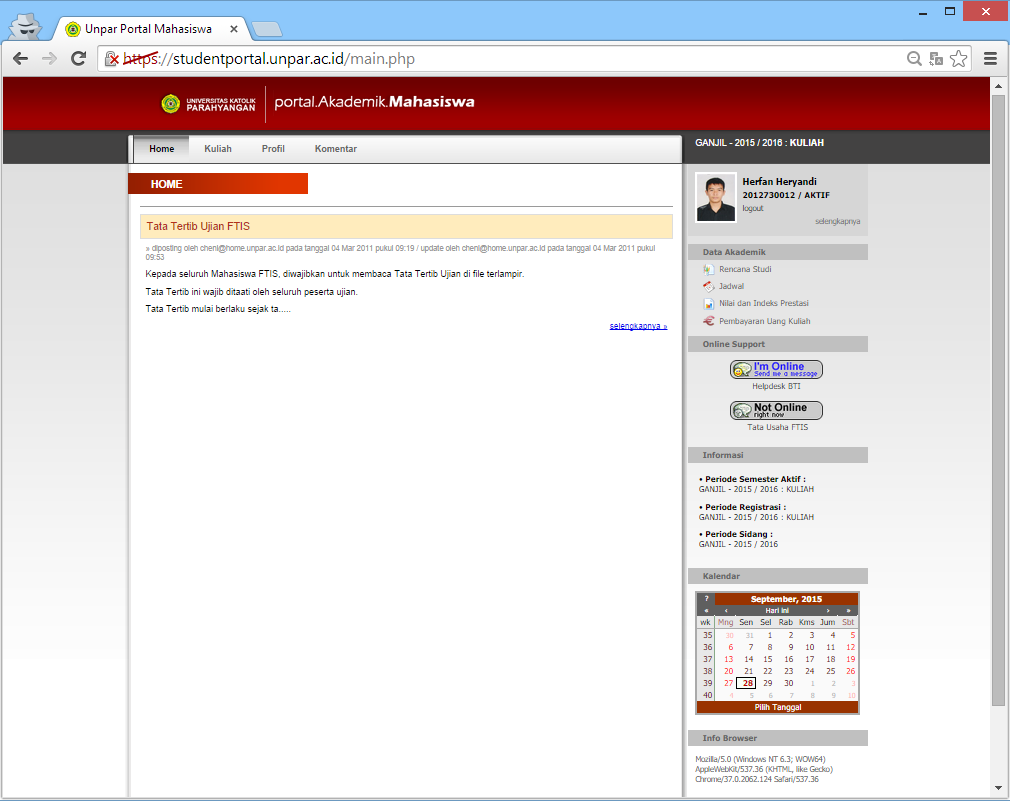
\includegraphics[scale=0.5]{Gambar/pam-home}
	\caption{Halaman Utama Portal Akademik Mahasiswa} 
	\label{fig:3_pam_home}
\end{figure}

Pada halaman utama Portal Akademik Mahasiswa (gambar \ref{fig:3_pam_home}), terdapat beberapa bagian yaitu:
\begin{enumerate}
	\item Menu Atas\\
	Menu ini berfungsi sebagai menu pendukung yang terdiri dari : 
	\begin{itemize}
		\item \textbf{Home}, menampilkan informasi atau pengumuman yang dikeluarkan oleh fakultas masing-masing (Gambar \ref{fig:3_pam_atas_home}). 
		
		\begin{figure}[H]
			\centering
			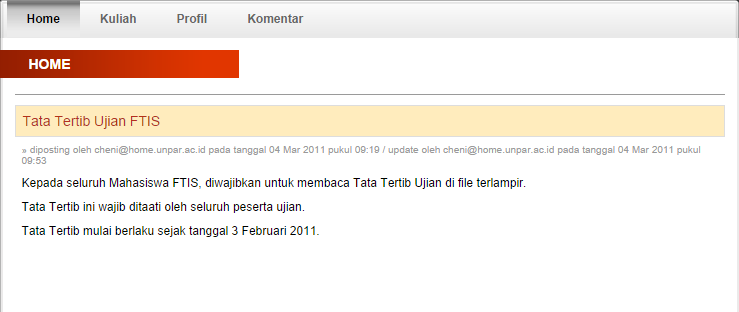
\includegraphics[scale=0.5]{Gambar/pam-atas-home}
			\caption{Menu Atas Home} 
			\label{fig:3_pam_atas_home}
		\end{figure}
		
		\item \textbf{Kuliah}, menampilkan pengumuman per mata kuliah sesuai dengan mata kuliah dan kelas yang diambil oleh masing-masing mahasiswa (Gambar \ref{fig:3_pam_atas_kuliah}).  
		
		\begin{figure}[H]
			\centering
			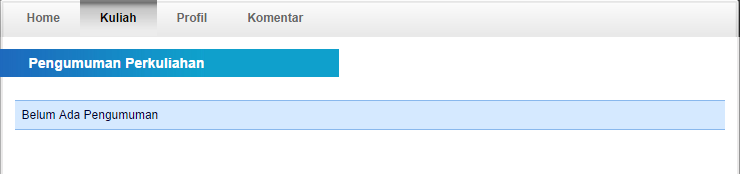
\includegraphics[scale=0.5]{Gambar/pam-atas-kuliah}
			\caption{Menu Atas Kuliah} 
			\label{fig:3_pam_atas_kuliah}
		\end{figure}
		
		\item \textbf{Profil}, berisi tentang data diri masing-masing mahasiswa (Gambar \ref{fig:3_pam_atas_profil}). 
		
		\begin{figure}[H]
			\centering
			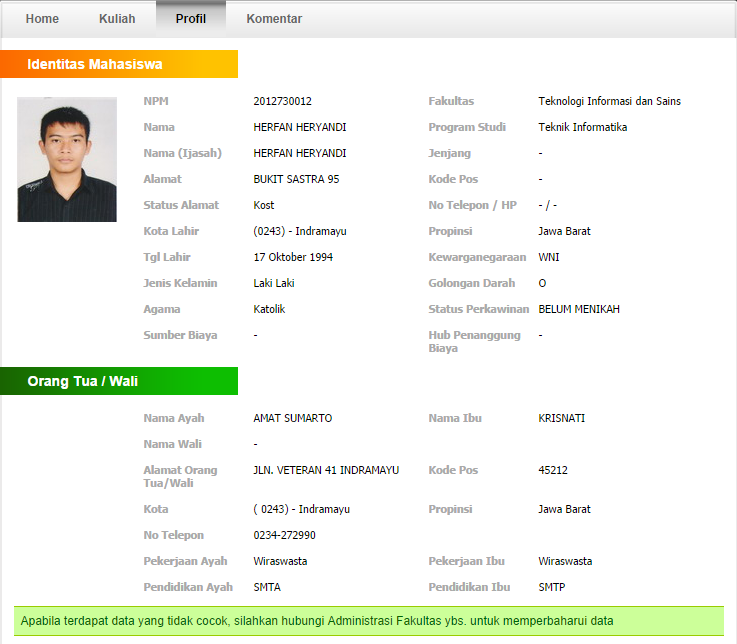
\includegraphics[scale=0.5]{Gambar/pam-atas-profil}
			\caption{Menu Atas Profil} 
			\label{fig:3_pam_atas_profil}
		\end{figure}
		
		\item \textbf{Komentar}, berisi komentar, saran, dan kritik dari mahasiswa (Gambar \ref{fig:3_pam_atas_komentar}).
		
		\begin{figure}[H]
			\centering
			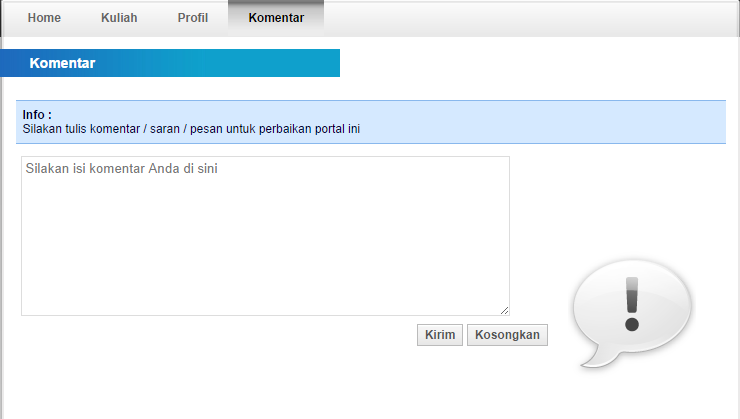
\includegraphics[scale=0.5]{Gambar/pam-atas-komentar}
			\caption{Menu Atas Komentar} 
			\label{fig:3_pam_atas_komentar}
		\end{figure}

	\end{itemize}
	
	\item Identitas Portal \\
	Bagian ini menampilkan identitas pengguna portal. Tampilan identitas ini dapat ditampilkan lengkap dengan melakukan klik pada \textit{link} ``selengkapnya'' atau ditampilkan minimal dengan klik \textit{link} ``tutup''. Identitas yang ditampilkan adalah nama, Nomor Pokok Mahasiswa (NPM), status keaktifan, pas foto, email, dosen wali, program studi, dan fakultas seperti yang terlihat pada gambar \ref{fig:3_pam_identitas}.   
	\begin{figure}[H]
			\centering
			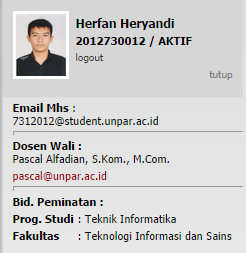
\includegraphics[scale=0.75]{Gambar/pam-identitas}
			\caption{Identitas Portal} 
			\label{fig:3_pam_identitas}
		\end{figure}
		
	\item Menu Utama\\
	Bagian ini memuat fitur utama Portal Akademik Mahasiswa mengenai data akademik (gambar \ref{fig:3_pam_utama}) yang terdiri dari:
		\begin{figure}[H]
			\centering
			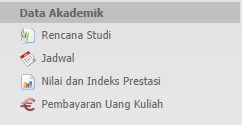
\includegraphics[scale=0.75]{Gambar/pam-utama}
			\caption{Menu Utama} 
			\label{fig:3_pam_utama}
		\end{figure}
	\begin{itemize}
	
		\item \textbf{Rencana Studi}\\
		Menu Rencana Studi terdiri dari submenu: 
		\begin{itemize}
			\item Registrasi (FRS/PRS)\\
			Digunakan sebagai formulir pengisian rencana studi awal (FRS) dan perubahan rencana studi (PRS) (Gambar \ref{fig:3_pam_utama_registrasi}). 			
			\begin{figure}[H]
				\centering
				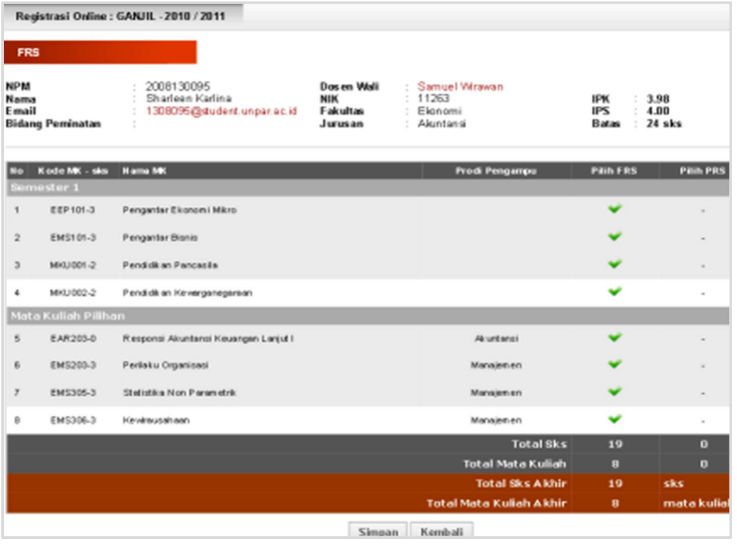
\includegraphics[scale=0.5]{Gambar/pam-utama-rencanastudi}
				\caption{Tampilan Registrasi FRS/PRS} 
				\label{fig:3_pam_utama_registrasi}
			\end{figure}
			
			\item Kartu Rencana Studi \\
			Menampilkan informasi mata kuliah yang telah diambil melalui submenu Registrasi (Gambar \ref{fig:3_pam_utama_krs}). Kartu Rencana Studi juga dapat dicetak melalui submenu ini. 
			\begin{figure}[H]
				\centering
				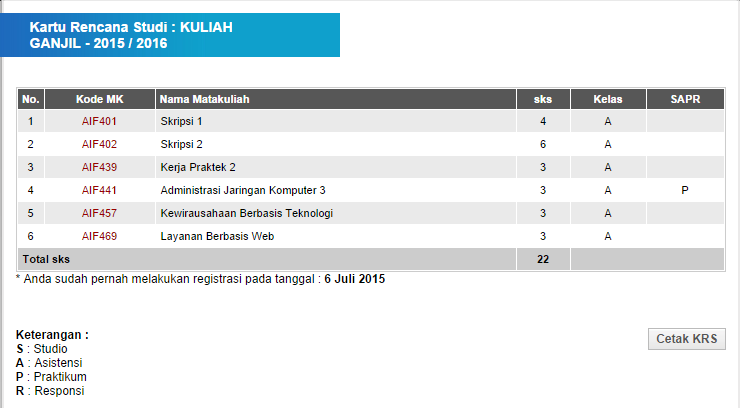
\includegraphics[scale=0.5]{Gambar/pam-utama-krs}
				\caption{Tampilan Kartu Rencana Studi\cite{BTI:2012}} 
				\label{fig:3_pam_utama_krs}
			\end{figure}
			
			\item Pindah Kelas MKU \\
			Mahasiswa dapat memilih kelas yang masih tersedia di kolom Jadwal Baru dan menekan tombol ``Simpan'' untuk setiap kelas yang diubah (Gambar \ref{fig:3_pam_utama_pindahmku}). 
			\begin{figure}[H]
				\centering
				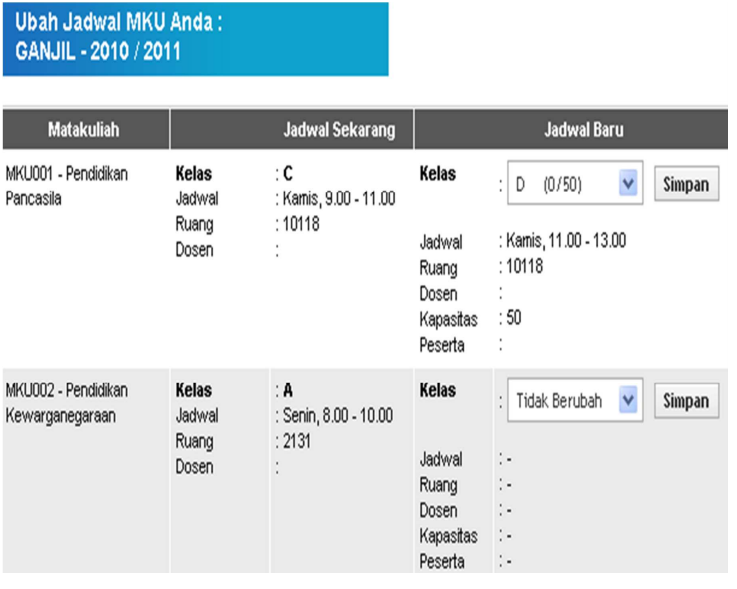
\includegraphics[scale=0.5]{Gambar/pam-utama-pindahmku}
				\caption{Tampilan Pindah Kelas MKU\cite{BTI:2012}} 
				\label{fig:3_pam_utama_pindahmku}
			\end{figure}

		\end{itemize}
		
		\item \textbf{ Jadwal}\\
		Menu Jadwal terdiri dari submenu: 
		\begin{itemize}
			\item Kuliah, UTS, dan UAS \\
			Submenu ini berisi tentang jadwal kuliah, UTS dan UAS yang dapat disusun per semester (Gambar \ref{fig:3_pam_utama_jadwal}). 
			\begin{figure}[H]
				\centering
				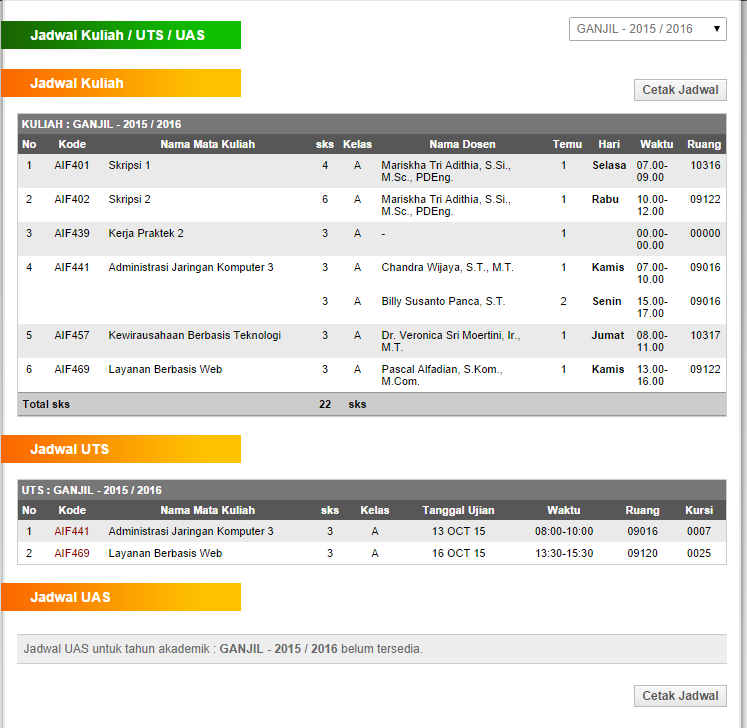
\includegraphics[scale=0.5]{Gambar/pam-utama-jadwal}
				\caption{Tampilan Jadwal Kuliah, UTS, dan UAS} 
				\label{fig:3_pam_utama_jadwal}
			\end{figure}
			
			\item MKU \\
			Submenu ini menampilkan seluruh jadwal Mata Kuliah Umum (MKU) yang memberikan informasi tentang kelas-kelas yang dibuka oleh Pusat Kajian Humaniora (PKH) (Gambar \ref{fig:3_pam_utama_jadwalmku}). 
			\begin{figure}[H]
				\centering
				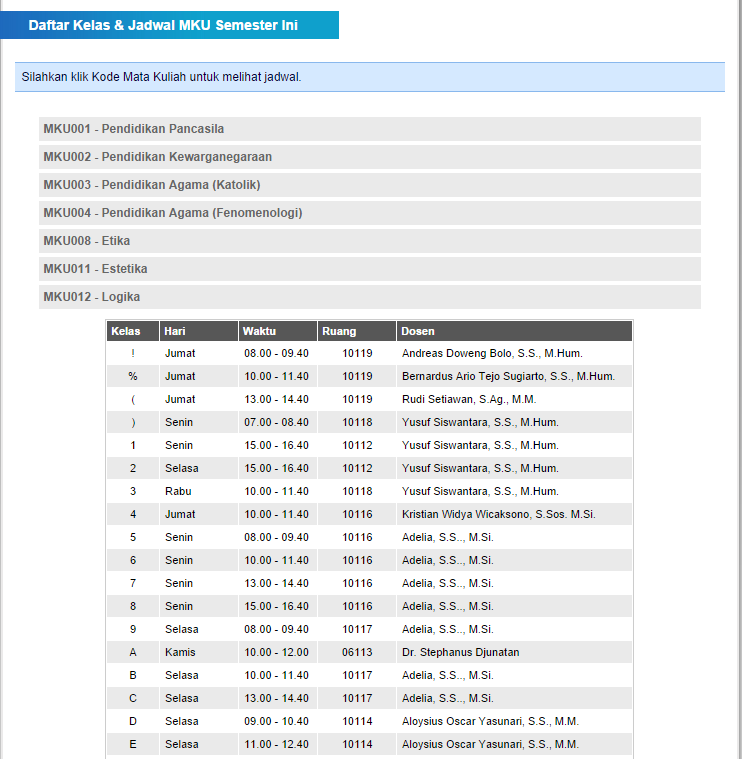
\includegraphics[scale=0.5]{Gambar/pam-utama-jadwalmku}
				\caption{Tampilan Jadwal MKU} 
				\label{fig:3_pam_utama_jadwalmku}
			\end{figure}
			
			\item Seluruh Fakultas \\
			Fitur ini memberikan informasi mengenai jadwal-jadwal yang ada di seluruh fakultas (Gambar \ref{fig:3_pam_utama_jadwalall}).
			\begin{figure}[H]
				\centering
				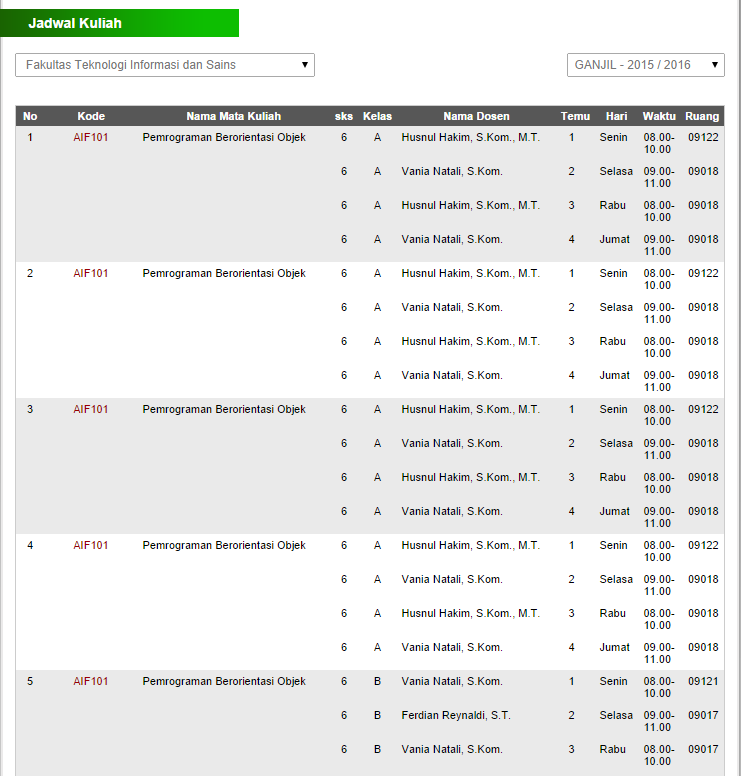
\includegraphics[scale=0.5]{Gambar/pam-utama-jadwalall}
				\caption{Tampilan Jadwal Seluruh Fakultas} 
				\label{fig:3_pam_utama_jadwalall}
			\end{figure}
		\end{itemize}
		
		\item \textbf{Nilai dan Indeks Prestasi}\\
		Menu Nilai dan Indeks Prestasi terdiri dari submenu: 
		\begin{itemize}
			\item Riwayat per Semester \\
			Submenu ini menampilkan informasi nilai per semester. Mahasiswa dapat melihat nilai sesuai dengan semester yang dipilih atau bisa memilih
pilihan ``Seluruh Tahun Akademik'' untuk melihat seluruh nilai berdasarkan semester (Gambar \ref{fig:3_pam_utama_nilai}).
			\begin{figure}[H]
				\centering
				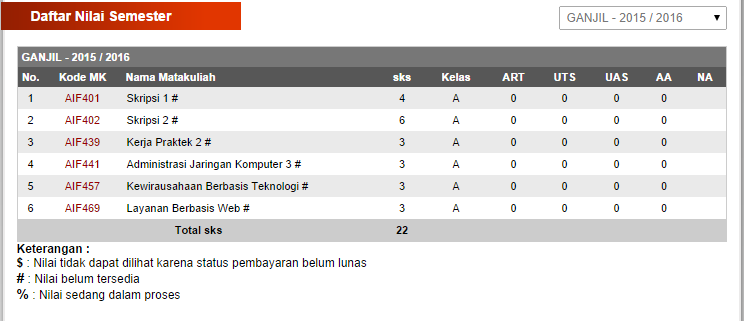
\includegraphics[scale=0.5]{Gambar/pam-utama-nilai}
				\caption{Tampilan Riwayat Per Semester} 
				\label{fig:3_pam_utama_nilai}
			\end{figure}
			
			\item Daftar Perkembangan Studi \\
			Seluruh riwayat mata kuliah dan nilai yang pernah ditempuh ditampilkan di submenu ini (Gambar \ref{fig:3_pam_utama_dps}). Pada bagian bawah halaman, terdapat statistik nilai dan indeks prestasi (Gambar \ref{fig:3_pam_utama_dpsstat}). 
			\begin{figure}[H]
				\centering
				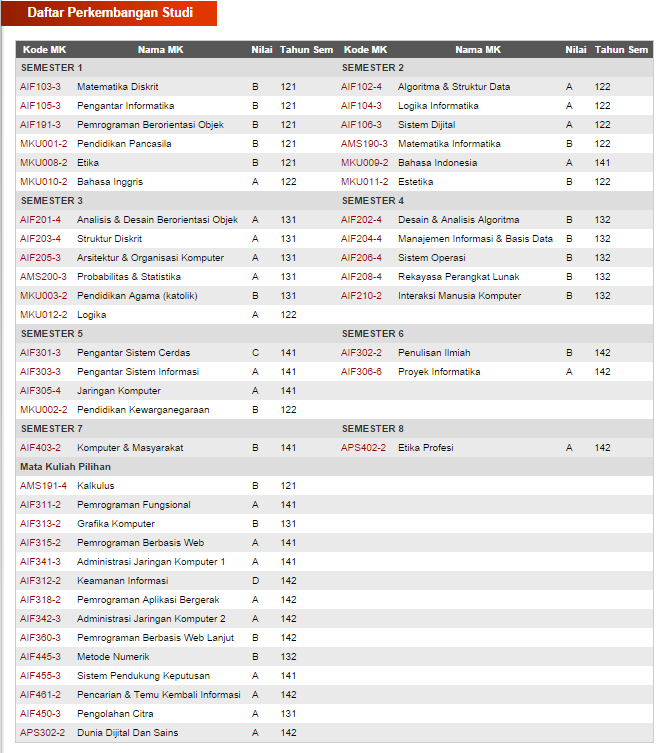
\includegraphics[scale=0.5]{Gambar/pam-utama-dps}
				\caption{Tampilan Daftar Perkembangan Studi} 
				\label{fig:3_pam_utama_dps}
			\end{figure}
			
			\begin{figure}[H]
				\centering
				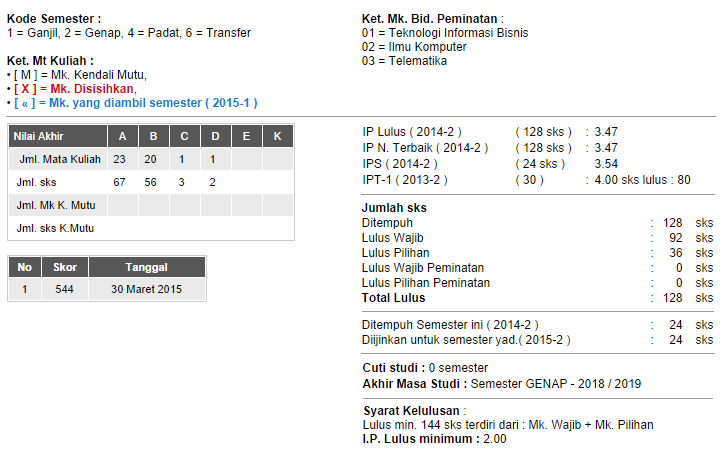
\includegraphics[scale=0.5]{Gambar/pam-utama-dpsstat}
				\caption{Tampilan Statistik Nilai dan IP} 
				\label{fig:3_pam_utama_dpsstat}
			\end{figure}
			
			\item Riwayat Indeks Prestasi \\
			Menampilkan daftar riwayat indeks prestasi semester dan kumulatif setiap semester. Tampilan ini juga dilengkapi dengan grafik perkembangan (Gambar \ref{fig:3_pam_utama_ip}). 
			\begin{figure}[H]
				\centering
				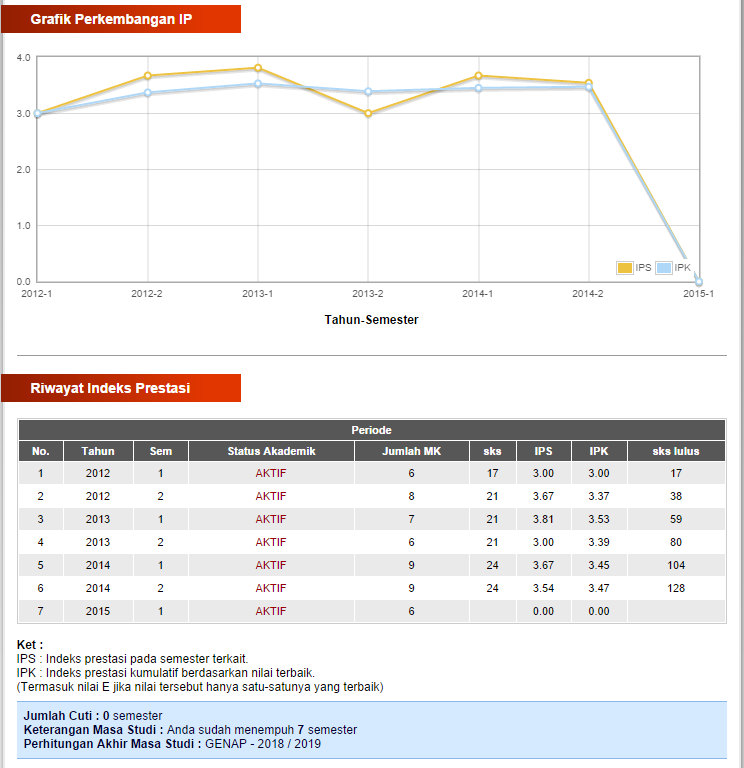
\includegraphics[scale=0.5]{Gambar/pam-utama-ip}
				\caption{Tampilan Riwayat Indeks Prestasi} 
				\label{fig:3_pam_utama_ip}
			\end{figure}
			
			\item TOEFL \\
			Menampilkan daftar riwayat skor \textit{Test of English as Foreign Language} (TOEFL) yang pernah ditempuh (Gambar \ref{fig:3_pam_utama_toefl}). Mahasiswa diwajibkan untuk menempuh TOEFL dengan skor minimal 500.
			
			\begin{figure}[H]
				\centering
				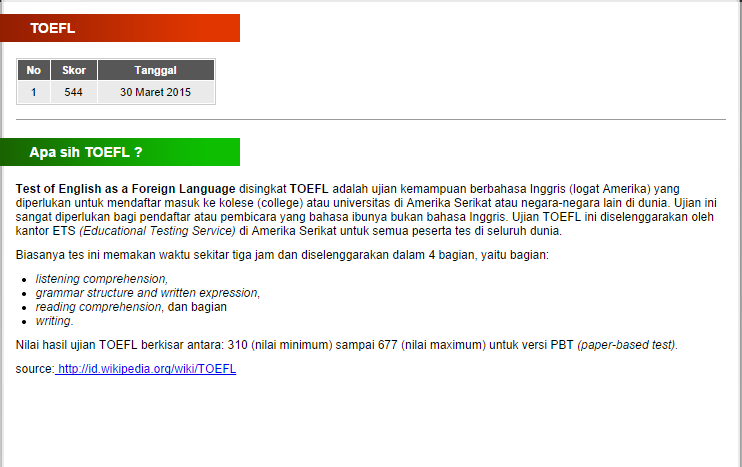
\includegraphics[scale=0.5]{Gambar/pam-utama-toefl}
				\caption{Tampilan TOEFL} 
				\label{fig:3_pam_utama_toefl}
			\end{figure}
		\end{itemize}
		
		\item \textbf{Pembayaran Uang Kuliah}\\
		Menu ini berfungsi untuk melihat data tagihan pembayaran uang kuliah serta cara-cara pembayarannya (Gambar \ref{fig:3_pam_utama_pembayaran}).
		\begin{figure}[H]
				\centering
				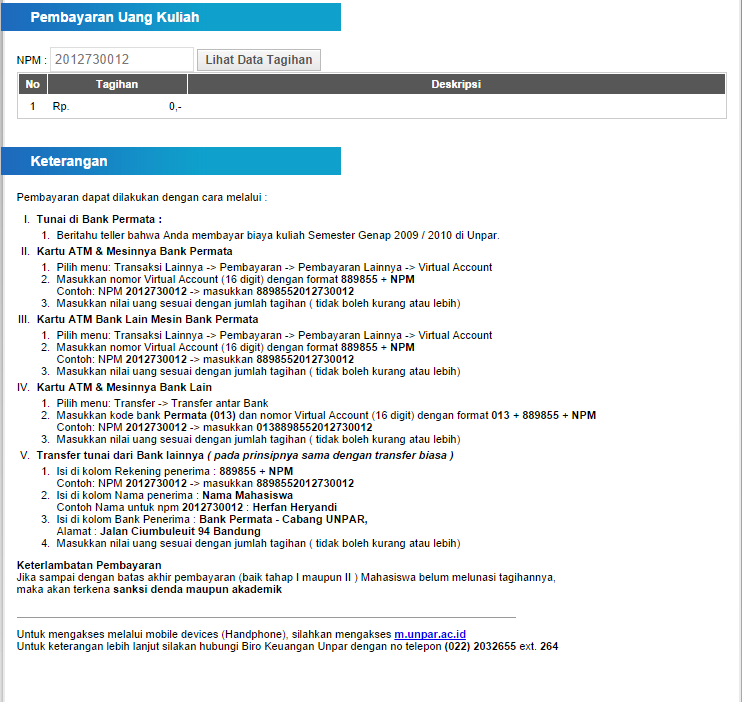
\includegraphics[scale=0.5]{Gambar/pam-utama-pembayaran}
				\caption{Tampilan Pembayaran Uang Kuliah} 
				\label{fig:3_pam_utama_pembayaran}
			\end{figure}
		\end{itemize}
		
	\item \textbf{Informasi}\\
		Bagian ini menampilkan informasi tentang periode-periode yang sedang aktif (Gambar \ref{fig:3_pam_utama_informasi}). Sebagai contoh jika ``Periode Registrasi'' diklik maka akan muncul \textit{pop up} seperti pada gambar \ref{fig:3_pam_utama_informasipop}.
			\begin{figure}[H]
				\centering
				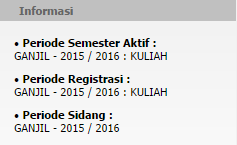
\includegraphics[scale=0.75]{Gambar/pam-utama-informasi}
				\caption{Tampilan Informasi} 
				\label{fig:3_pam_utama_informasi}
			\end{figure}
			
			\begin{figure}[H]
				\centering
				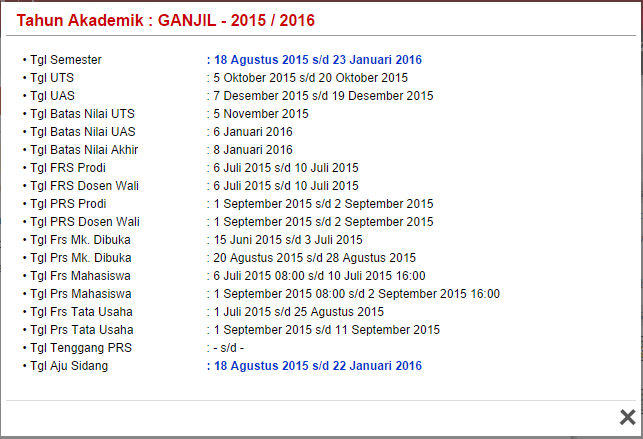
\includegraphics[scale=0.5]{Gambar/pam-utama-infopop}
				\caption{Tampilan \textit{Pop Up} Informasi} 
				\label{fig:3_pam_utama_informasipop}
			\end{figure}
		
	\item \textbf{Kalender}\\
		Bagian ini menampilkan kalender masehi (Gambar \ref{fig:3_pam_utama_kalender}).
		\begin{figure}[H]
				\centering
				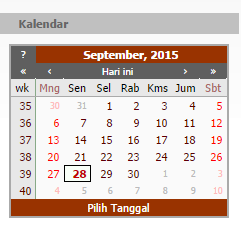
\includegraphics[scale=0.75]{Gambar/pam-utama-kalender}
				\caption{Tampilan Kalender} 
				\label{fig:3_pam_utama_kalender}
			\end{figure}
		
	\item \textbf{Info Browser}\\
		Bagian ini menampilkan informasi tentang internet \textit{browser} yang digunakan pada saat membuka Portal Akademik Mahasiswa (Gambar \ref{fig:3_pam_utama_infobrowser}). 
		\begin{figure}[H]
				\centering
				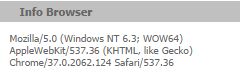
\includegraphics[scale=0.75]{Gambar/pam-utama-infobrowser}
				\caption{Tampilan Info Browser} 
				\label{fig:3_pam_utama_infobrowser}
			\end{figure}
\end{enumerate}

\item\textbf{Analisis Komunikasi Portal Akademik Mahasiswa untuk Fitur IT Student Portal}
Untuk memenuhi fitur IT Student Portal, penulis menganalisis komunikasi Portal Akademik Mahasiswa ke dalam beberapa kasus yang akan dijelaskan pada bagian-bagian berikut.

\textbf{Kasus \textit{Login}}\\
Di Portal Akademik Mahasiswa, mahasiswa dapat \textit{login} dengan cara:
\begin{enumerate}
	\item Mengakses \url{https://studentportal.unpar.ac.id/} dan mengklik tombol ``input\#submit.login-button'' (Gambar \ref{fig:3_case_login}).
	\begin{figure}[H]
			\centering
			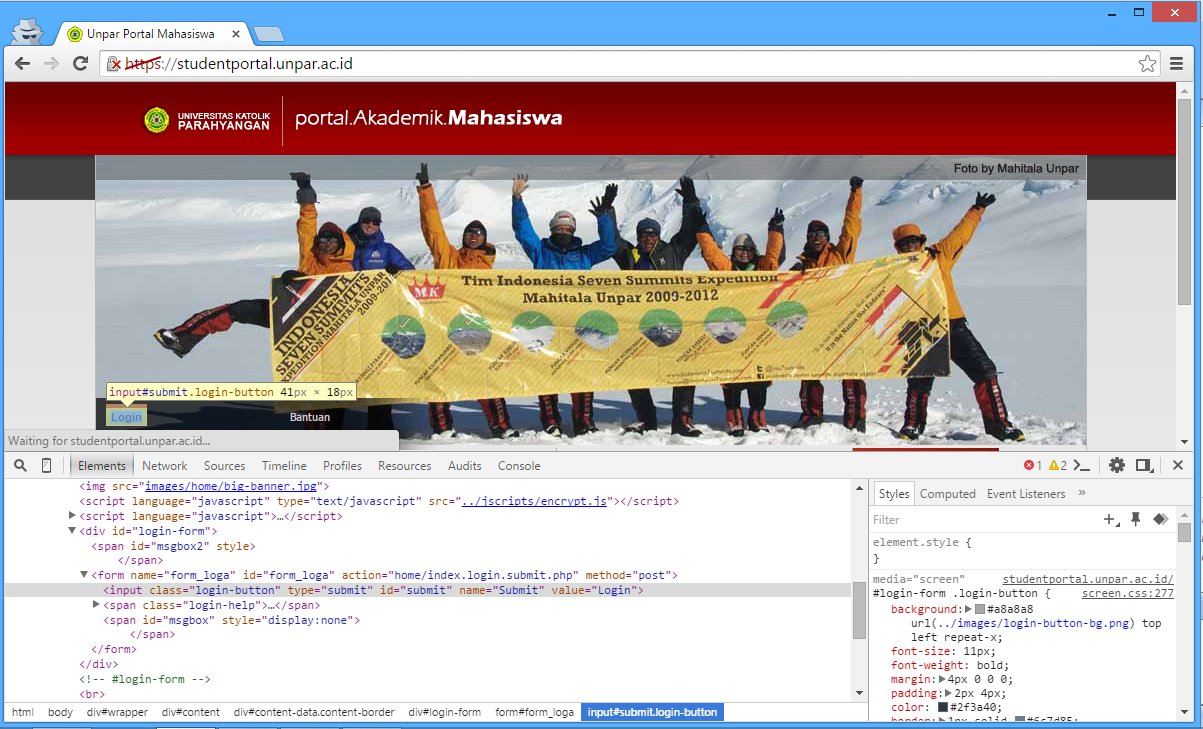
\includegraphics[scale=0.5]{Gambar/case-login}
			\caption{Tombol ``input\#submit.login-button'' pada Halaman Depan Portal Akademik Mahasiswa} 
			\label{fig:3_case_login}
		\end{figure}
		
	\item Saat tombol tersebut ditekan, mahasiswa akan dibawa ke halaman \url{index.login.submit.php} dengan \textit{form data} berisi:
			\begin{itemize}
				\item Submit: selalu berisi ``Login''
			\end{itemize}
		
	\item Secara otomatis halaman akan berpindah lagi ke \url{https://cas.unpar.ac.id/login? service=https\%3A\%2F\%2Fstudentportal.unpar.ac.id\%2Fhome\%2Findex.login.submit.php}.
		
	\item Di sana, akan ditampilkan halaman \textit{login} CAS UNPAR di mana mahasiswa diminta mengisi \textit{``Username''} pada kolom ``input\#username.required'' dan \textit{``Password''} pada kolom ``input\#password.required'' (Gambar \ref{fig:3_case_login_cas}).
	\begin{figure}[H]
			\centering
			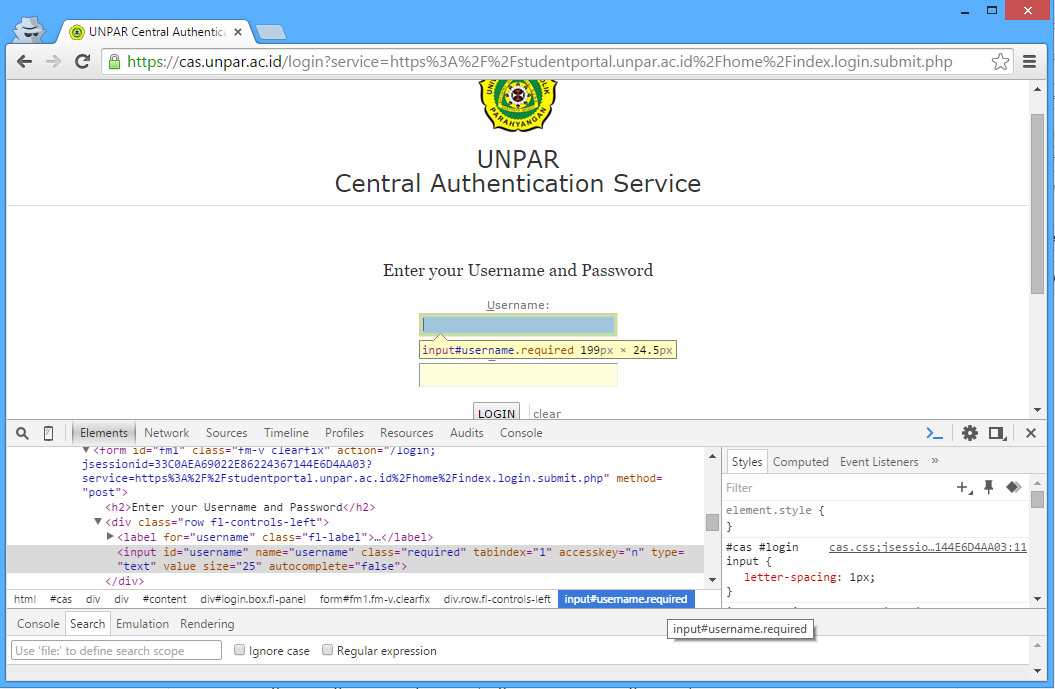
\includegraphics[scale=0.5]{Gambar/case-login-cas}
			\caption{Kolom \textit{``Username''} ``input\#username.required'' pada Halaman CAS UNPAR} 
			\label{fig:3_case_login_cas}
		\end{figure}
	\item Setelah itu mahasiswa harus menekan tombol ``input.btn-submit''. Data tersebut akan dikirimkan ke \url{/login;jsessionid=...?service=https://studentportal.unpar.ac.id/home/index.login.submit.php} dengan \textit{cookie}:
	\begin{itemize}
		\item JSESSIONID: diambil dari \textit{cookie} yang di-\textit{set} pada halaman \url{https://cas.unpar.ac.id/login? service=https\%3A\%2F\%2Fstudentportal.unpar.ac.id\%2Fhome\%2Findex.login.submit.php}
	\end{itemize}
	 Data yang dikirim juga mengandung \textit{form data} sebagai berikut (Gambar \ref{fig:3_case_form}):
	\begin{itemize}
		\item username: diambil dari nilai elemen ``input\#username.required''
		\item password: diambil dari nilai elemen ``input\#password.required''
		\item lt: diambil dari nilai elemen ``input'' dengan nama ``lt''
		\item execution: diambil dari nilai elemen ``input'' dengan nama ``execution''
		\item \_eventId: selalu berisi ``submit''
		\item submit: selalu berisi ``LOGIN''
		\begin{figure}[H]
			\centering
			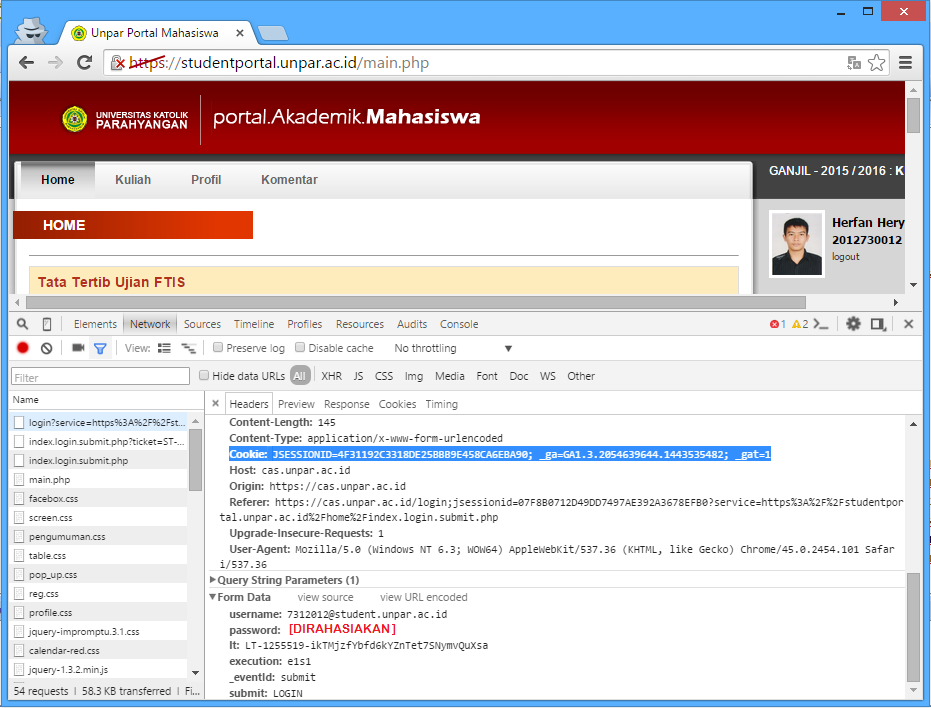
\includegraphics[scale=0.5]{Gambar/case-form}
			\caption{\textit{Form Data} yang dikirim CAS UNPAR} 
			\label{fig:3_case_form}
		\end{figure}
	\end{itemize}
\item Jika berhasil, akan dilakukan pengalihan beberapa kali dan diakhiri di \url{https://studentportal.unpar.ac.id/main.php} dengan \textit{cookie} sebagai berikut:
\begin{itemize}
	\item PHPSESSID: diambil dari \textit{cookie} yang di-\textit{set} pada beberapa pengalihan sebelumnya
	\item \_ga dan \_gat: tidak diperlukan, digunakan oleh Google Analytics\footnote{\url{https://developers.google.com/analytics/devguides/collection/analyticsjs/cookie-usage}}
\end{itemize}
\end{enumerate}

\textbf{Kasus Nilai}\\
Di halaman utama Portal Akademik Mahasiswa, mahasiswa dapat melihat riwayat nilai dengan cara:
\begin{enumerate}
	\item Mengklik ``a.first-line-menu'' dengan teks ``Nilai dan Indeks Prestasi'' 
	\item Setelah diklik, akan muncul list ``ul.hidden'', kemudian mahasiswa harus mengklik elemen ``a'' dengan teks ``Riwayat Per Semester'' (Gambar \ref{fig:3_case_nilai_menu})
	\begin{figure}[H]
			\centering
			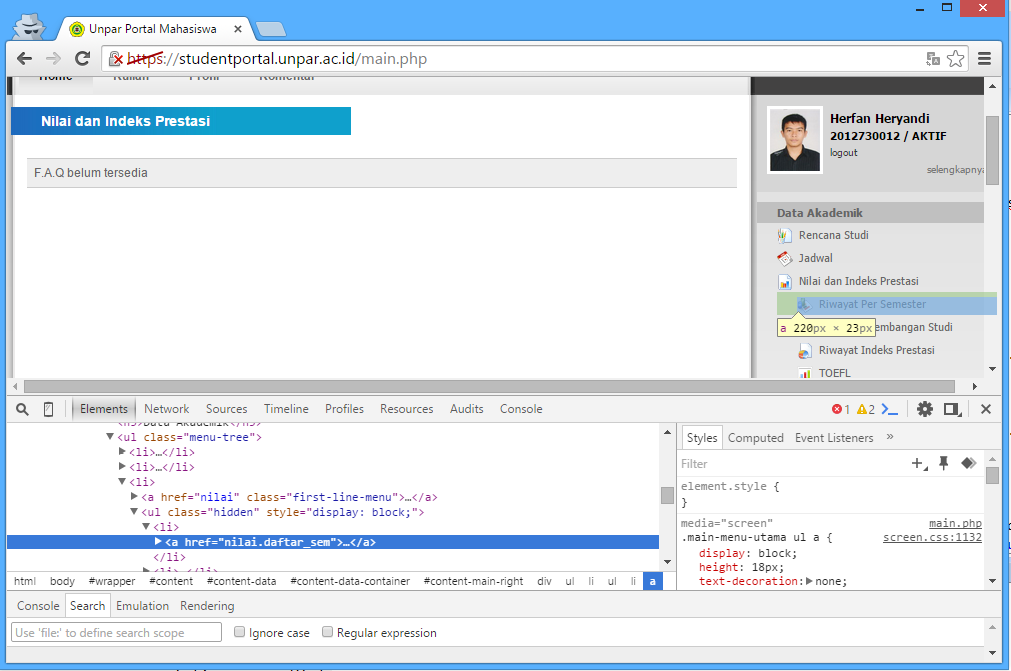
\includegraphics[scale=0.5]{Gambar/case-nilai-menu}
			\caption{Elemen ``a'' dengan teks ``Riwayat Per Semester'' pada Menu Nilai dan Indeks Prestasi} 
			\label{fig:3_case_nilai_menu}
		\end{figure}
		\item Setelah mengklik ``Riwayat Per Semester'', mahasiswa akan diarahkan ke \url{https://studentportal.unpar.ac.id/includes/nilai.daftar_sem.php} dengan \textit{cookie} sebagai berikut:
\begin{itemize}
	\item PHPSESSID: diambil dari \textit{cookie} yang di-\textit{set} saat pengalihan ke halaman utama
\end{itemize}
		\item Halaman ``Riwayat Per Semester'' menampilkan nilai semester terkini. Jika ingin melihat nilai semester sebelumnya, mahasiswa dapat mengklik \textit{combo box} ``select\#tahun\_akd\_sec'' kemudian memilih ``option'' yang diinginkan atau ``Seluruh Tahun Akademik'' untuk melihat nilai seluruh semester (Gambar \ref{fig:3_case_nilai_pilih}).
		
		\begin{figure}[H]
			\centering
			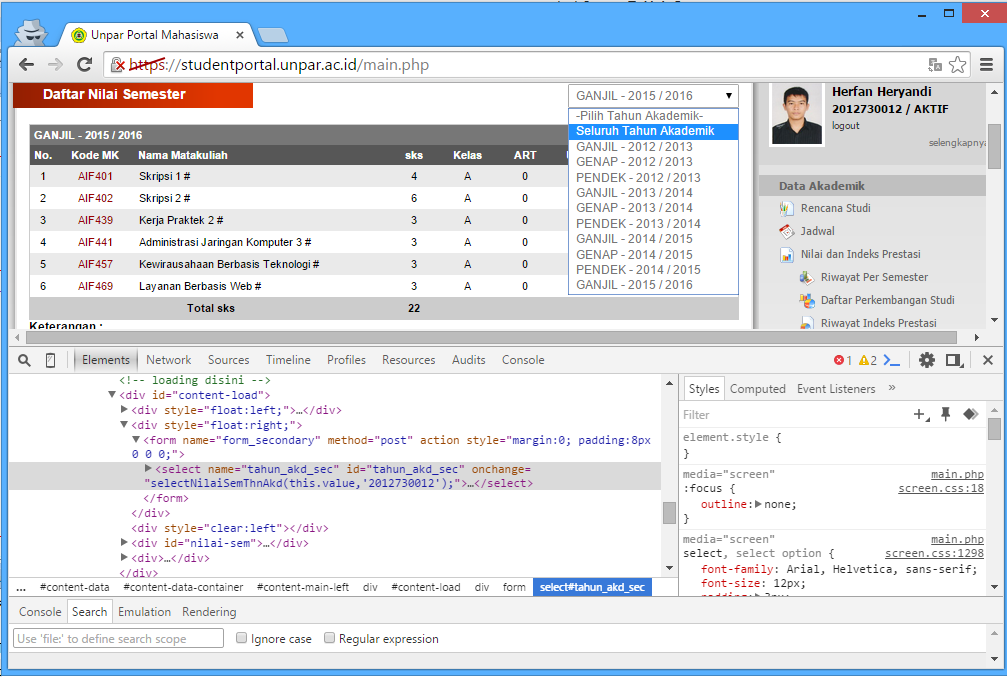
\includegraphics[scale=0.5]{Gambar/case-nilai-pilih}
			\caption{\textit{Combo Box} ``select\#tahun\_akd\_sec'' pada Halaman Riwayat Per Semester} 
			\label{fig:3_case_nilai_pilih}
		\end{figure}
		
		\item  Setelah memilih ``option'', mahasiswa akan dibawa ke \url{https://studentportal.unpar.ac.id/includes/nilai.sem.php} (Gambar \ref{fig:3_case_nilai}) dengan \textit{cookie} PHPSESSID dan mengandung \textit{form data}:
		\begin{itemize}
			\item npm: diperoleh dari NPM mahasiswa
			\item thn\_akd: berisi tahun akademik semester atau berisi ``ALL'' jika memilih ``Seluruh Tahun Akademik''
			\item sem\_akd: berisi semester akademik dalam angka (1: ganjil, 2: genap, 4: pendek) atau tidak didefinisikan jika memilih ``Seluruh Tahun Akademik''
		\end{itemize}
		
		\begin{figure}[H]
			\centering
			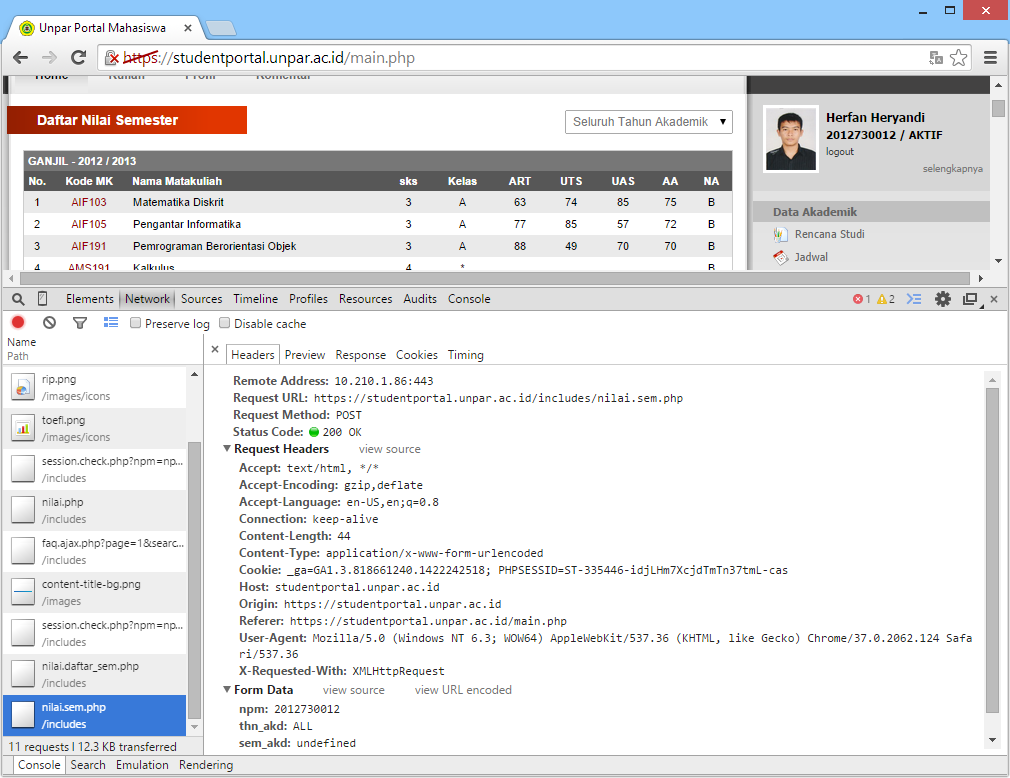
\includegraphics[scale=0.5]{Gambar/case-nilai}
			\caption{\textit{Form Data} pada pengiriman Nilai Seluruh Tahun Akademik} 
			\label{fig:3_case_nilai}
		\end{figure}
\end{enumerate}

\textbf{Kasus Jadwal}\\
Di halaman utama Portal Akademik Mahasiswa, mahasiswa dapat melihat jadwal dengan cara:
\begin{enumerate}
	\item Mengklik ``a.first-line-menu'' dengan teks ``Jadwal'' 
	\item Setelah diklik, akan muncul list ``ul.hidden'', kemudian mahasiswa harus mengklik elemen ``a'' dengan teks ``Kuliah, UTS dan UAS''(Gambar \ref{fig:3_case_jadwal_menu})
	\begin{figure}[H]
			\centering
			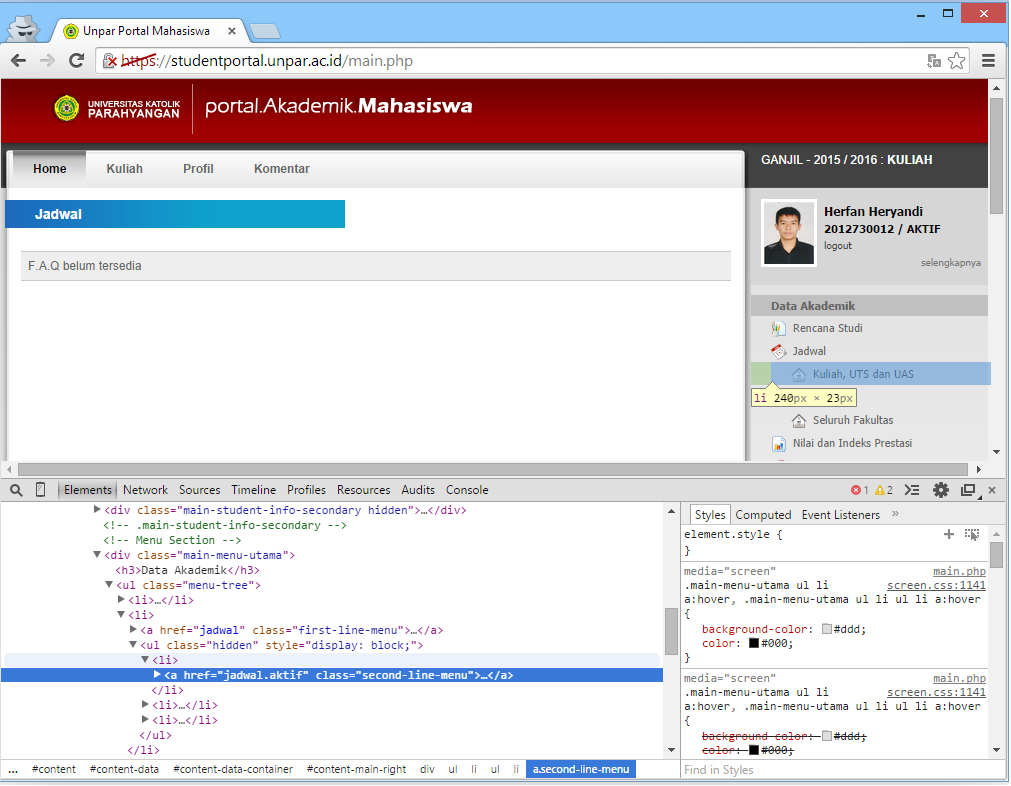
\includegraphics[scale=0.5]{Gambar/case-jadwal-menu}
			\caption{Elemen ``a'' dengan teks ``Kuliah, UTS dan UAS'' pada Menu Jadwal} 
			\label{fig:3_case_jadwal_menu}
		\end{figure}
		\item Setelah mengklik ``Kuliah, UTS dan UAS'', mahasiswa akan diarahkan ke \url{https://studentportal.unpar.ac.id/includes/jadwal.aktif.php} dengan \textit{cookie} sebagai berikut:
\begin{itemize}
	\item PHPSESSID: diambil dari \textit{cookie} yang di-\textit{set} saat pengalihan ke halaman utama
\end{itemize}
\item Halaman ``Kuliah, UTS dan UAS'' menampilkan jadwal kuliah, UTS, dan UAS semester terkini. Jika ingin melihat jadwal semester sebelumnya, mahasiswa dapat mengklik \textit{combo box} ``select\#tahun\_akd\_sec'' kemudian memilih ``option'' yang diinginkan (Gambar \ref{fig:3_case_jadwal_pilih}).
		
		\begin{figure}[H]
			\centering
			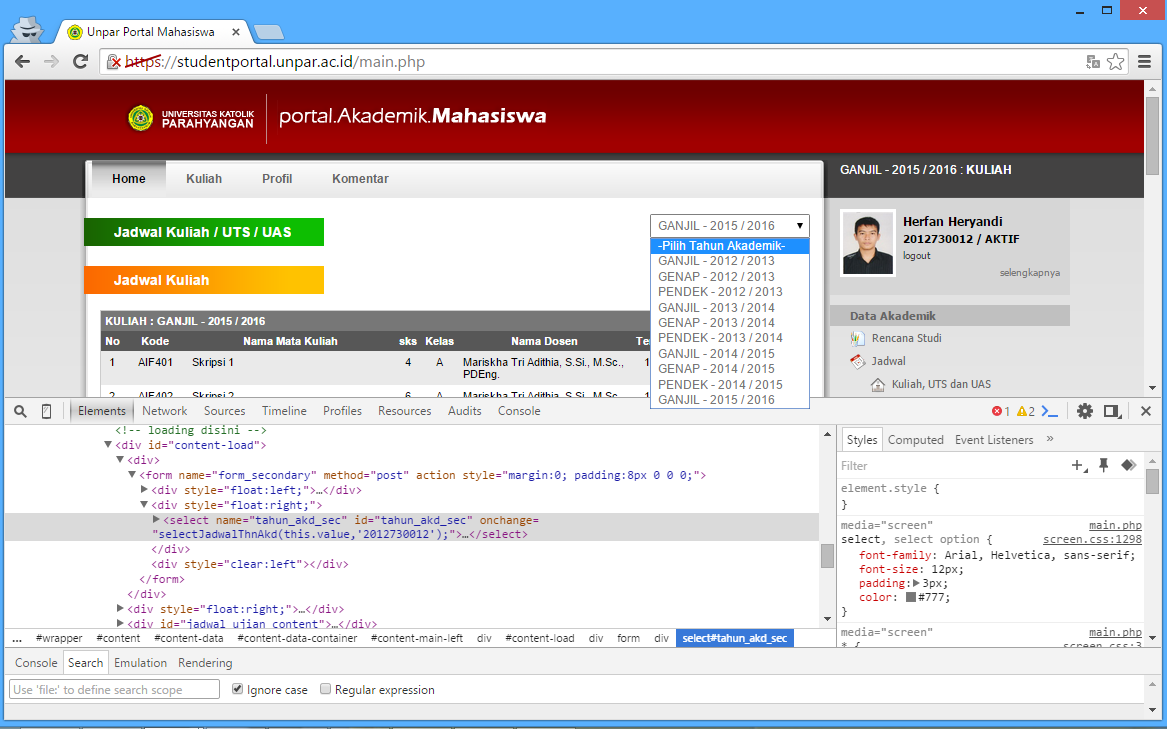
\includegraphics[scale=0.5]{Gambar/case-jadwal-pilih}
			\caption{Combo Box ``select\#tahun\_akd\_sec'' pada Halaman Jadwal Kuliah, UTS, dan UAS} 
			\label{fig:3_case_jadwal_pilih}
		\end{figure}
		
		\item  Setelah memilih ``option'', mahasiswa akan ditampilkan jawaban dari \url{https://studentportal.unpar.ac.id/includes/jadwal.kuliah.php} dan \url{https://studentportal.unpar.ac.id/includes/jadwal.ujian.php} (Gambar \ref{fig:3_case_jadwal}) dengan \textit{cookie} PHPSESSID dan mengandung \textit{form data}:
		\begin{itemize}
			\item npm: diperoleh dari NPM mahasiswa
			\item thn\_akd: berisi tahun akademik semester 
			\item sem\_akd: berisi semester akademik dalam angka (1: ganjil, 2: genap, 4: pendek) 
		\end{itemize}
		
		\begin{figure}[H]
			\centering
			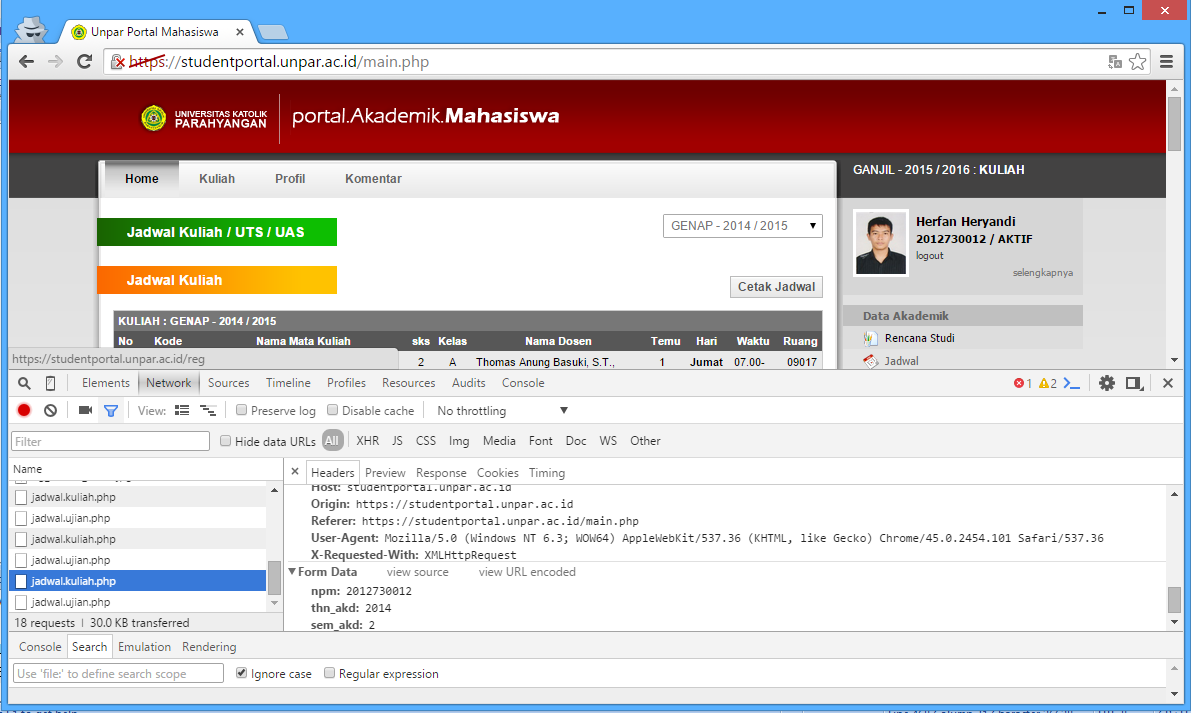
\includegraphics[scale=0.5]{Gambar/case-jadwal}
			\caption{\textit{Form Data} pada pengiriman Jadwal Kuliah dan Ujian} 
			\label{fig:3_case_jadwal}
		\end{figure}
		
\end{enumerate}

Mahasiswa juga dapat melihat jadwal seluruh fakultas dengan cara:
\begin{enumerate}
	\item Mengklik ``a.second-line-menu'' dengan teks ``Seluruh Fakultas'' pada \textit{list} ``ul.hidden'' (Gambar \ref{fig:3_case_jadwal_seluruh})
	\begin{figure}[H]
			\centering
			\includegraphics[scale=0.5]{Gambar/case-jadwal-seluruh}
			\caption{Elemen ``a'' dengan teks ``Seluruh Fakultas'' pada Menu Jadwal} 
			\label{fig:3_case_jadwal_seluruh}
		\end{figure}
	\item Setelah diklik, mahasiswa akan diarahkan ke \url{https://studentportal.unpar.ac.id/includes/jadwal.all.php} dengan \textit{cookie} sebagai berikut:
\begin{itemize}
	\item PHPSESSID: diambil dari \textit{cookie} yang di-\textit{set} saat pengalihan ke halaman utama
\end{itemize}
		\item Halaman ``Seluruh Fakultas'' menampilkan seluruh jadwal semester terkini pada fakultas tempat mahasiswa menempuh studi. Jika ingin melihat jadwal semester sebelumnya, mahasiswa dapat mengklik \textit{combo box} ``select\#tahun\_akd\_sec'' kemudian memilih ``option'' yang diinginkan. Jika ingin melihat jadwal fakultas lain, mahasiswa dapat mengklik \textit{combo box} ``select\#jadwal\_all\_ps'' kemudian memilih ``option'' fakultas yang diinginkan (Gambar \ref{fig:3_case_jadwal_pilihfak}).
		\begin{figure}[H]
			\centering
			\includegraphics[scale=0.5]{Gambar/case-jadwal-pilihfak}
			\caption{Combo Box ``select\#jadwal\_all\_ps'' pada Halaman Jadwal Seluruh Fakultas} 
			\label{fig:3_case_jadwal_pilihfak}
		\end{figure}
		\item  Setelah memilih ``option'', mahasiswa akan dibawa ke \url{https://studentportal.unpar.ac.id/includes/jadwal.all.content.php}(Gambar \ref{fig:3_case_jadwal_fakultas}) dengan \textit{cookie} PHPSESSID dan mengandung \textit{query string parameter}:
		\begin{itemize}
			\item kode\_fak: berisi kode fakultas 
			\item thn\_akd: berisi tahun akademik semester 
			\item sem\_akd: berisi semester akademik dalam angka (1: ganjil, 2: genap, 4: pendek) 
		\end{itemize}
		
		\begin{figure}[H]
			\centering
			\includegraphics[scale=0.5]{Gambar/case-jadwal-fakultas}
			\caption{\textit{Form Data} pada pengiriman Jadwal Seluruh Fakultas} 
			\label{fig:3_case_jadwal_fakultas}
		\end{figure}
\end{enumerate}

\textbf{Kasus \textit{Logout}}\\
Mahasiswa dapat melakukan \textit{logout} dengan cara:
\begin{enumerate}
	\item Mengklik ``a'' dengan teks ``logout'' pada bagian identitas portal (Gambar \ref{fig:3_case_logout_link})
	\begin{figure}[H]
			\centering
			\includegraphics[scale=0.5]{Gambar/case-logout-link}
			\caption{Elemen ``a'' dengan teks ``logout'' pada Identitas Portal} 
			\label{fig:3_case_logout_link}
		\end{figure}
	\item Setelah diklik, mahasiswa akan diarahkan ke \url{https://studentportal.unpar.ac.id/home/index.logout.php} dengan \textit{cookie} sebagai berikut:
		\begin{itemize}
			\item PHPSESSID: diambil dari \textit{cookie} yang di-\textit{set} saat pengalihan ke halaman utama
		\end{itemize} 
	\item Kemudian dilakukan pengalihan ke \url{https://cas.unpar.ac.id/logout?service=https\%3A\%2F\%2Fstudentportal.unpar.ac.id} lalu mengadaluarsakan \textit{cookie} CASTGC dan CASPRIVACY yang sebelumnya di-\textit{set} saat pengalihan ke halaman utama (Gambar \ref{fig:3_case_logout_expires}) 
			\begin{figure}[H]
				\centering
				\includegraphics[scale=0.5]{Gambar/case-logout-expires}
				\caption{Pengadaluarsaan Cookie CASTGC dan CASPRIVACY} 
				\label{fig:3_case_logout_expires}
			\end{figure}
		\item Pengalihan diakhiri di \url{https://studentportal.unpar.ac.id/} yaitu halaman depan Portal Akademik Mahasiswa (Gambar \ref{fig:3_case_logout}) 
		\begin{figure}[H]
				\centering
				\includegraphics[scale=0.5]{Gambar/case-logout}
				\caption{Pengalihan ke Halaman Depan Portal Akademik Mahasiswa} 
				\label{fig:3_case_logout}
			\end{figure}
\end{enumerate}

\item \textbf{Analisis \textit{Use Case}}\\
\textbf{Diagram \textit{Use Case}}\\
Diagram \textit{use case} pada perangkat lunak yang akan dibangun hanya mengandung satu aktor, yaitu mahasiswa. Diagram \textit{use case} dapat dilihat pada gambar \ref{fig:3_usecase_diagram}. 
		\begin{figure}[H]
			\centering
			\includegraphics[scale=0.5]{Gambar/usecase-diagram}
			\caption{Diagram \textit{Use Case} IT Student Portal} 
			\label{fig:3_usecase_diagram}
		\end{figure}
Berdasarkan hasil analisis wawancara, dari lima fitur yang akan dibuat, dibentuk tiga \textit{use case} antara lain:
\begin{itemize}
	\item \textbf{Memeriksa Prasyarat Mata Kuliah}, mahasiswa dapat memeriksa mata kuliah yang dibuka pada semester terkini apakah memenuhi prasyarat atau tidak. 
	\item \textbf{Melihat Jadwal Kuliah, UTS, dan UAS}, mahasiswa dapat melihat jadwal kuliah, UTS, dan UAS yang sudah tersusun dan terurut berdasarkan hari.
	\item \textbf{Melihat Ringkasan Data Akademik}, mahasiswa dapat melihat data mengenai mata kuliah apa saja yang sudah lulus beserta jenis mata kuliahnya(wajib, pilihan, atau pilihan wajib), sisa SKS untuk mencapai kelulusan, dan mata kuliah wajib yang belum ditempuh. Mahasiswa juga dapat melihat IPS dan IPK yang berubah berdasarkan riwayat nilai.
\end{itemize}

\textbf{Skenario \textit{Use Case}}\\

\begin{enumerate}
	\item \textbf{Memeriksa Prasyarat Mata Kuliah}
		\begin{itemize}
			\item Nama: Memeriksa prasyarat mata kuliah
			\item Aktor: Mahasiswa
			\item Deskripsi: Memeriksa prasyarat mata kuliah yang dibuka pada semester terkini
			\item Kondisi awal: Mahasiswa telah \textit{login}
			\item Kondisi akhir: Halaman prasyarat mata kuliah ditampilkan dan berisi prasyarat mata kuliah yang dibuka pada semester terkini
			\item Skenario utama: \\ \\
				\begin{tabular}{|p{0.5cm} |p{6cm}| p{6cm}|}
						\hline
							No 	& Aksi Aktor & Reaksi Sistem \\ \hline
							1 	& Mahasiswa memilih menu prasyarat mata kuliah. 	&	Sistem mendapatkan data mahasiswa kemudian menampilkan halaman prasyarat mata kuliah \\ \hline 
						\end{tabular} 
			\item Eksepsi: -
		\end{itemize}
		
	\item \textbf{Melihat Jadwal Kuliah, UTS, dan UAS}
		\begin{itemize}
			\item Nama: Melihat jadwal kuliah, UTS, dan UAS
			\item Aktor: Mahasiswa
			\item Deskripsi: Melihat jadwal kuliah, UTS, dan UAS yang sudah tersusun dan terurut berdasarkan hari
			\item Kondisi awal: Mahasiswa telah \textit{login}
			\item Kondisi akhir: Halaman jadwal ditampilkan dan berisi jadwal kuliah, UTS, dan UAS yang sudah tersusun dan terurut berdasarkan hari te
			\item Skenario utama: \\ \\
				\begin{tabular}{|p{0.5cm} |p{6cm}| p{6cm}|}
						\hline
							No 	& Aksi Aktor & Reaksi Sistem \\ \hline
							1 	& Mahasiswa memilih menu jadwal. 	&	Sistem menyusun dan mengurutkan jadwal mahasiswa berdasarkan hari kemudian menampilkan halaman jadwal \\ \hline 
						\end{tabular} 
			\item Eksepsi: Mahasiswa sedang cuti studi
		\end{itemize}
		
	\item \textbf{Melihat Ringkasan Data Akademik}
		\begin{itemize}
			\item Nama: Melihat ringkasan data akademik
			\item Aktor: Mahasiswa
			\item Deskripsi: melihat data mengenai mata kuliah apa saja yang sudah lulus beserta jenis mata kuliahnya(wajib, pilihan, atau pilihan wajib), sisa SKS untuk mencapai kelulusan, dan mata kuliah wajib yang belum ditempuh. Mahasiswa juga dapat melihat IPS dan IPK yang berubah berdasarkan riwayat nilai
			\item Kondisi awal: Mahasiswa telah \textit{login}
			\item Kondisi akhir: Halaman jadwal ditampilkan dan berisi jadwal ringkasan data akademik
			\item Skenario utama: \\ \\
			\begin{tabular}{|p{0.5cm} |p{6cm}| p{6cm}|}
						\hline
							No 	& Aksi Aktor & Reaksi Sistem \\ \hline
							1 	& Mahasiswa memilih menu ringkasan data akademik. 	&	Sistem meringkas data kademik mahasiswa kemudian menampilkan halaman ringkasan data akademik \\ \hline 
						\end{tabular} 
			\item Eksepsi: -
		\end{itemize}
\end{enumerate}

\item{Analisis Kelas}
Diagram kelas analisis untuk IT Student Portal ditunjukkan pada gambar \ref{fig:3_class_diagram}.
	\begin{figure}[H]
			\centering
			\includegraphics[scale=0.5]{Gambar/class-diagram}
			\caption{Diagram Kelas Analisis IT Student Portal} 
			\label{fig:3_class_diagram}
		\end{figure}
Kelas-kelas dari \textit{package} SIA Models telah dibahas pada poin 1 bagian SIA Models. Sedangkan penjelasan dari kelas-kelas lainnya sebagai berikut:
\begin{enumerate}
	\item Controller\\
	Kelas ini merupakan kelas yang sudah disediakan oleh Play Framework. Turunan dari kelas ini akan berperan sebagai \textit{controller}.
	\item Application\\
	Kelas ini merupakan \textit{controller} pada IT Student Portal yang berfungsi untuk menghubungkan \textit{model} dengan \textit{view}. 
	\item Scraper\\
	Kelas ini merupakan kelas yang mengimplementasikan \textit{web scraping} menggunakan \textit{library} jsoup. Kelas ini digunakan untuk memperoleh data dari Portal Akademik Mahasiswa kemudian menghubungkannya ke dalam SIA Models. Data-data yang sudah dihubungkan dengan SIA Models akan ditampilkan ke \textit{view} melalui kelas \texttt{Application}.
\end{enumerate}
			\end{enumerate}

		\item Mengimplementasikan \textit{web scraping} menggunakan \textit{library} jsoup.\\
		{\bf status :} Ada sejak rencana kerja skripsi.\\
		{\bf hasil :} -
		\item Membangun perangkat lunak IT Student Portal.\\
		{\bf status :} Ada sejak rencana kerja skripsi.\\
		{\bf hasil :} -

		\item Melakukan eksperimen dan pengujian\\
		{\bf status :} Ada sejak rencana kerja skripsi.\\
		{\bf hasil :} -

		\item Menulis dokumen skripsi\\
		{\bf status :} Ada sejak rencana kerja skripsi.\\
		{\bf hasil :} Dokumen skripsi sudah ditulis hingga bab 3.


\end{enumerate}


\bibliographystyle{ieeetr}
\bibliography{pustaka}

\section{Pencapaian Rencana Kerja}
Persentase penyelesaian skripsi sampai dengan dokumen ini dibuat dapat dilihat pada tabel berikut :

\begin{center}
  \begin{tabular}{ | c | c | c | c | l | c |}
    \hline
    1*  & 2*(\%) & 3*(\%) & 4*(\%) &5* &6*(\%)\\ \hline \hline
   1   & 14  & 14  &  &  & 13\\ \hline
    2   & 14 & 14  &   &  & 14\\ \hline
    3   & 14  & 14  &  &  & 14\\ \hline
    4   & 14  &   &  14 &  & \\ \hline
    5   & 14  &   & 14 &  & \\ \hline
    6   & 14 &   & 14  &  & \\ \hline
    7   & 16  & 8  & 8 &  {\footnotesize bab 1, bab 2, dan bab 3 di S1} & 8\\ \hline
    Total  & 100  & 50  & 50 &  & 49\\ \hline
                          \end{tabular}										
\end{center}

Keterangan (*)\\
1 : Bagian pengerjaan Skripsi (nomor disesuaikan dengan detail pengerjaan di bagian 5)\\
2 : Persentase total \\
3 : Persentase yang akan diselesaikan di Skripsi 1 \\
4 : Persentase yang akan diselesaikan di Skripsi 2 \\
5 : Penjelasan singkat apa yang dilakukan di S1 (Skripsi 1) atau S2 (skripsi 2)\\
6 : Persentase yang sudah diselesaikan sampai saat ini 

%\section{Kendala yang dihadapi}
%TULISKAN BAGIAN INI JIKA DOKUMEN ANDA TIPE A ATAU C
%Kendala - kendala yang dihadapi selama mengerjakan skripsi :
%\begin{itemize}
%	\item Terlalu banyak melakukan prokratinasi
%	\item Mengalami kesulitan dalam instalasi Play Framework
%	\item Kurang familiar dengan pemrograman Play Framework
%\end{itemize}

\vspace{1cm}
\centering Bandung, \tanggal\\
\vspace{2cm} \nama \\ 
\vspace{1cm}

Menyetujui, \\
\ifdefstring{\jumpemb}{2}{
\vspace{1.5cm}
\begin{centering} Menyetujui,\\ \end{centering} \vspace{0.75cm}
\begin{minipage}[b]{0.45\linewidth}
% \centering Bandung, \makebox[0.5cm]{\hrulefill}/\makebox[0.5cm]{\hrulefill}/2013 \\
\vspace{2cm} Nama: \pembA \\ Pembimbing Utama
\end{minipage} \hspace{0.5cm}
\begin{minipage}[b]{0.45\linewidth}
% \centering Bandung, \makebox[0.5cm]{\hrulefill}/\makebox[0.5cm]{\hrulefill}/2013\\
\vspace{2cm} Nama: \pemB \\ Pembimbing Pendamping
\end{minipage}
\vspace{0.3cm}
}{
% \centering Bandung, \makebox[0.5cm]{\hrulefill}/\makebox[0.5cm]{\hrulefill}/2013\\
\vspace{2cm} Nama: \pembA \\ Pembimbing Tunggal
}
`
\end{document}

